\documentclass[twoside]{book}

% Packages required by doxygen
\usepackage{fixltx2e}
\usepackage{calc}
\usepackage{doxygen}
\usepackage[export]{adjustbox} % also loads graphicx
\usepackage{graphicx}
\usepackage[utf8]{inputenc}
\usepackage{makeidx}
\usepackage{multicol}
\usepackage{multirow}
\PassOptionsToPackage{warn}{textcomp}
\usepackage{textcomp}
\usepackage[nointegrals]{wasysym}
\usepackage[table]{xcolor}

% Font selection
\usepackage[T1]{fontenc}
\usepackage[scaled=.90]{helvet}
\usepackage{courier}
\usepackage{amssymb}
\usepackage{sectsty}
\renewcommand{\familydefault}{\sfdefault}
\allsectionsfont{%
  \fontseries{bc}\selectfont%
  \color{darkgray}%
}
\renewcommand{\DoxyLabelFont}{%
  \fontseries{bc}\selectfont%
  \color{darkgray}%
}
\newcommand{\+}{\discretionary{\mbox{\scriptsize$\hookleftarrow$}}{}{}}

% Page & text layout
\usepackage{geometry}
\geometry{%
  a4paper,%
  top=2.5cm,%
  bottom=2.5cm,%
  left=2.5cm,%
  right=2.5cm%
}
\tolerance=750
\hfuzz=15pt
\hbadness=750
\setlength{\emergencystretch}{15pt}
\setlength{\parindent}{0cm}
\setlength{\parskip}{3ex plus 2ex minus 2ex}
\makeatletter
\renewcommand{\paragraph}{%
  \@startsection{paragraph}{4}{0ex}{-1.0ex}{1.0ex}{%
    \normalfont\normalsize\bfseries\SS@parafont%
  }%
}
\renewcommand{\subparagraph}{%
  \@startsection{subparagraph}{5}{0ex}{-1.0ex}{1.0ex}{%
    \normalfont\normalsize\bfseries\SS@subparafont%
  }%
}
\makeatother

% Headers & footers
\usepackage{fancyhdr}
\pagestyle{fancyplain}
\fancyhead[LE]{\fancyplain{}{\bfseries\thepage}}
\fancyhead[CE]{\fancyplain{}{}}
\fancyhead[RE]{\fancyplain{}{\bfseries\leftmark}}
\fancyhead[LO]{\fancyplain{}{\bfseries\rightmark}}
\fancyhead[CO]{\fancyplain{}{}}
\fancyhead[RO]{\fancyplain{}{\bfseries\thepage}}
\fancyfoot[LE]{\fancyplain{}{}}
\fancyfoot[CE]{\fancyplain{}{}}
\fancyfoot[RE]{\fancyplain{}{\bfseries\scriptsize Generated by Doxygen }}
\fancyfoot[LO]{\fancyplain{}{\bfseries\scriptsize Generated by Doxygen }}
\fancyfoot[CO]{\fancyplain{}{}}
\fancyfoot[RO]{\fancyplain{}{}}
\renewcommand{\footrulewidth}{0.4pt}
\renewcommand{\chaptermark}[1]{%
  \markboth{#1}{}%
}
\renewcommand{\sectionmark}[1]{%
  \markright{\thesection\ #1}%
}

% Indices & bibliography
\usepackage{natbib}
\usepackage[titles]{tocloft}
\setcounter{tocdepth}{3}
\setcounter{secnumdepth}{5}
\makeindex

% Hyperlinks (required, but should be loaded last)
\usepackage{ifpdf}
\ifpdf
  \usepackage[pdftex,pagebackref=true]{hyperref}
\else
  \usepackage[ps2pdf,pagebackref=true]{hyperref}
\fi
\hypersetup{%
  colorlinks=true,%
  linkcolor=blue,%
  citecolor=blue,%
  unicode%
}

% Custom commands
\newcommand{\clearemptydoublepage}{%
  \newpage{\pagestyle{empty}\cleardoublepage}%
}

\usepackage{caption}
\captionsetup{labelsep=space,justification=centering,font={bf},singlelinecheck=off,skip=4pt,position=top}

%===== C O N T E N T S =====

\begin{document}

% Titlepage & ToC
\hypersetup{pageanchor=false,
             bookmarksnumbered=true,
             pdfencoding=unicode
            }
\pagenumbering{alph}
\begin{titlepage}
\vspace*{7cm}
\begin{center}%
{\Large Reference Manual}\\
\vspace*{1cm}
{\large Generated by Doxygen 1.8.14}\\
\end{center}
\end{titlepage}
\clearemptydoublepage
\pagenumbering{roman}
\tableofcontents
\clearemptydoublepage
\pagenumbering{arabic}
\hypersetup{pageanchor=true}

%--- Begin generated contents ---
\chapter{Description}
\label{index}\hypertarget{index}{}S\+EP Projekt zu Flashkaskaden 
\chapter{Hierarchical Index}
\section{Class Hierarchy}
This inheritance list is sorted roughly, but not completely, alphabetically\+:\begin{DoxyCompactList}
\item \contentsline{section}{cascade$<$ TS, NP, NS, TP $>$}{\pageref{classcascade}}{}
\item \contentsline{section}{L\+I\+N\+E\+A\+R\+\_\+\+S\+O\+L\+V\+ER$<$ TA, N, Tb, Tx $>$}{\pageref{class_l_i_n_e_a_r___s_o_l_v_e_r}}{}
\begin{DoxyCompactList}
\item \contentsline{section}{LU$<$ TA, N, Tb, Tx $>$}{\pageref{class_l_u}}{}
\item \contentsline{section}{QR$<$ TA, N, Tb, Tx $>$}{\pageref{class_q_r}}{}
\end{DoxyCompactList}
\item \contentsline{section}{L\+I\+N\+E\+A\+R\+\_\+\+S\+O\+L\+V\+ER$<$ TS, NS $>$}{\pageref{class_l_i_n_e_a_r___s_o_l_v_e_r}}{}
\item \contentsline{section}{L\+I\+N\+E\+A\+R\+\_\+\+S\+Y\+S\+T\+EM$<$ TA, N, Tb, Tx $>$}{\pageref{class_l_i_n_e_a_r___s_y_s_t_e_m}}{}
\item \contentsline{section}{Module$<$ TS, NP, NS, TP $>$}{\pageref{class_module}}{}
\item \contentsline{section}{Module$<$$>$}{\pageref{class_module}}{}
\begin{DoxyCompactList}
\item \contentsline{section}{Flash$<$ TS, NP, NS, TP $>$}{\pageref{class_flash}}{}
\end{DoxyCompactList}
\item \contentsline{section}{M\+O\+D\+U\+L\+E\+N\+E\+W\+T\+ON$<$ TS, NP, NS, TP $>$}{\pageref{class_m_o_d_u_l_e_n_e_w_t_o_n}}{}
\item \contentsline{section}{N\+O\+N\+L\+I\+N\+E\+A\+R\+\_\+\+S\+O\+L\+V\+ER$<$ TS, NP, NS, TP $>$}{\pageref{class_n_o_n_l_i_n_e_a_r___s_o_l_v_e_r}}{}
\begin{DoxyCompactList}
\item \contentsline{section}{N\+E\+W\+T\+ON$<$ TS, NP, NS, TP $>$}{\pageref{class_n_e_w_t_o_n}}{}
\end{DoxyCompactList}
\item \contentsline{section}{N\+O\+N\+L\+I\+N\+E\+A\+R\+\_\+\+S\+Y\+S\+T\+EM$<$ TS, NP, NS, TP $>$}{\pageref{class_n_o_n_l_i_n_e_a_r___s_y_s_t_e_m}}{}
\item Q\+Main\+Window\begin{DoxyCompactList}
\item \contentsline{section}{Main\+Window}{\pageref{class_main_window}}{}
\end{DoxyCompactList}
\item \contentsline{section}{Test\+Class}{\pageref{class_test_class}}{}
\end{DoxyCompactList}

\chapter{Class Index}
\section{Class List}
Here are the classes, structs, unions and interfaces with brief descriptions\+:\begin{DoxyCompactList}
\item\contentsline{section}{\mbox{\hyperlink{classcascade}{cascade$<$ Real\+Type $>$}} \\*Enthält alle Flashes }{\pageref{classcascade}}{}
\item\contentsline{section}{\mbox{\hyperlink{class_c_a_s_c_a_d_e_e_s_o}{C\+A\+S\+C\+A\+D\+E\+E\+SO}} }{\pageref{class_c_a_s_c_a_d_e_e_s_o}}{}
\item\contentsline{section}{\mbox{\hyperlink{class_flash}{Flash$<$ Real\+Type $>$}} \\*Flashmodul }{\pageref{class_flash}}{}
\item\contentsline{section}{\mbox{\hyperlink{class_l_i_n_e_a_r___s_o_l_v_e_r}{L\+I\+N\+E\+A\+R\+\_\+\+S\+O\+L\+V\+E\+R$<$ T\+A, N, Tb, Tx $>$}} }{\pageref{class_l_i_n_e_a_r___s_o_l_v_e_r}}{}
\item\contentsline{section}{\mbox{\hyperlink{class_l_i_n_e_a_r___s_y_s_t_e_m}{L\+I\+N\+E\+A\+R\+\_\+\+S\+Y\+S\+T\+E\+M$<$ T\+A, N, Tb, Tx $>$}} \\*Lineare Systeme Basierend auf \mbox{\hyperlink{lin__sys_8h}{lin\+\_\+sys.\+h}} von Uwe Naumann }{\pageref{class_l_i_n_e_a_r___s_y_s_t_e_m}}{}
\item\contentsline{section}{\mbox{\hyperlink{class_l_u}{L\+U$<$ T\+A, N, Tb, Tx $>$}} }{\pageref{class_l_u}}{}
\item\contentsline{section}{\mbox{\hyperlink{class_module}{Module$<$ Real\+Type $>$}} \\*Akstrakte Klasse für allgemeine Bauteile }{\pageref{class_module}}{}
\item\contentsline{section}{\mbox{\hyperlink{class_n_e_w_t_o_n}{N\+E\+W\+T\+O\+N$<$ T\+S, N\+P, N\+S, T\+P $>$}} }{\pageref{class_n_e_w_t_o_n}}{}
\item\contentsline{section}{\mbox{\hyperlink{class_n_o_n_l_i_n_e_a_r___s_o_l_v_e_r}{N\+O\+N\+L\+I\+N\+E\+A\+R\+\_\+\+S\+O\+L\+V\+E\+R$<$ T\+S, N\+P, N\+S, T\+P $>$}} }{\pageref{class_n_o_n_l_i_n_e_a_r___s_o_l_v_e_r}}{}
\item\contentsline{section}{\mbox{\hyperlink{class_n_o_n_l_i_n_e_a_r___s_y_s_t_e_m}{N\+O\+N\+L\+I\+N\+E\+A\+R\+\_\+\+S\+Y\+S\+T\+E\+M$<$ T\+S, N\+P, N\+S, T\+P $>$}} \\*Nichtlineare Systeme Basierend auf \mbox{\hyperlink{nonlin__sys_8h}{nonlin\+\_\+sys.\+h}} von Uwe Naumann }{\pageref{class_n_o_n_l_i_n_e_a_r___s_y_s_t_e_m}}{}
\item\contentsline{section}{\mbox{\hyperlink{class_q_r}{Q\+R$<$ T\+A, N, Tb, Tx $>$}} }{\pageref{class_q_r}}{}
\item\contentsline{section}{\mbox{\hyperlink{class_world_machine}{World\+Machine}} \\*C++ -\/ Q\+ML Schnittstelle Organisiert die Kaskade und das G\+UI }{\pageref{class_world_machine}}{}
\end{DoxyCompactList}

\chapter{File Index}
\section{File List}
Here is a list of all files with brief descriptions\+:\begin{DoxyCompactList}
\item\contentsline{section}{\mbox{\hyperlink{cascade_8h}{cascade.\+h}} \\*Enthält alle \mbox{\hyperlink{class_module}{Module}} }{\pageref{cascade_8h}}{}
\item\contentsline{section}{\mbox{\hyperlink{flash_8h}{flash.\+h}} \\*\mbox{\hyperlink{class_flash}{Flash}} als Erweiterung des Moduls }{\pageref{flash_8h}}{}
\item\contentsline{section}{\mbox{\hyperlink{lin__sys_8h}{lin\+\_\+sys.\+h}} \\*Lineare Systeme }{\pageref{lin__sys_8h}}{}
\item\contentsline{section}{\mbox{\hyperlink{main_8cpp}{main.\+cpp}} \\*Main funcion }{\pageref{main_8cpp}}{}
\item\contentsline{section}{\mbox{\hyperlink{mainwindow_8cpp}{mainwindow.\+cpp}} \\*Hauptfenster }{\pageref{mainwindow_8cpp}}{}
\item\contentsline{section}{\mbox{\hyperlink{mainwindow_8h}{mainwindow.\+h}} \\*Hauptfenster }{\pageref{mainwindow_8h}}{}
\item\contentsline{section}{\mbox{\hyperlink{module_8h}{module.\+h}} \\*Basismodul }{\pageref{module_8h}}{}
\item\contentsline{section}{\mbox{\hyperlink{nonlin__sys_8h}{nonlin\+\_\+sys.\+h}} \\*Nichtlineare Systeme }{\pageref{nonlin__sys_8h}}{}
\item\contentsline{section}{\mbox{\hyperlink{testclass_8h}{testclass.\+h}} }{\pageref{testclass_8h}}{}
\end{DoxyCompactList}

\chapter{Class Documentation}
\hypertarget{classcascade}{}\section{cascade Class Reference}
\label{classcascade}\index{cascade@{cascade}}


Enthält alle Flashes.  




{\ttfamily \#include $<$cascade.\+h$>$}

\subsection*{Public Member Functions}
\begin{DoxyCompactItemize}
\item 
\mbox{\hyperlink{classcascade_a0215d853ce25d724cd778ab512b0eda6}{cascade}} ()
\begin{DoxyCompactList}\small\item\em Konstruktor. \end{DoxyCompactList}\end{DoxyCompactItemize}


\subsection{Detailed Description}
Enthält alle Flashes. 

\subsection{Constructor \& Destructor Documentation}
\mbox{\Hypertarget{classcascade_a0215d853ce25d724cd778ab512b0eda6}\label{classcascade_a0215d853ce25d724cd778ab512b0eda6}} 
\index{cascade@{cascade}!cascade@{cascade}}
\index{cascade@{cascade}!cascade@{cascade}}
\subsubsection{\texorpdfstring{cascade()}{cascade()}}
{\footnotesize\ttfamily cascade\+::cascade (\begin{DoxyParamCaption}{ }\end{DoxyParamCaption})}



Konstruktor. 



The documentation for this class was generated from the following files\+:\begin{DoxyCompactItemize}
\item 
\mbox{\hyperlink{cascade_8h}{cascade.\+h}}\item 
\mbox{\hyperlink{cascade_8cpp}{cascade.\+cpp}}\end{DoxyCompactItemize}

\hypertarget{class_c_a_s_c_a_d_e_e_s_o}{}\section{C\+A\+S\+C\+A\+D\+E\+E\+SO Class Reference}
\label{class_c_a_s_c_a_d_e_e_s_o}\index{C\+A\+S\+C\+A\+D\+E\+E\+SO@{C\+A\+S\+C\+A\+D\+E\+E\+SO}}


{\ttfamily \#include $<$cascade.\+h$>$}

\subsection*{Public Member Functions}
\begin{DoxyCompactItemize}
\item 
\mbox{\hyperlink{class_c_a_s_c_a_d_e_e_s_o_a602657637f64c2c16d9b2141165afc11}{C\+A\+S\+C\+A\+D\+E\+E\+SO}} ()
\item 
void \mbox{\hyperlink{class_c_a_s_c_a_d_e_e_s_o_a87ddbb1f74cbb26db6dafa7d780ed7e9}{solve}} ()
\end{DoxyCompactItemize}


\subsection{Constructor \& Destructor Documentation}
\mbox{\Hypertarget{class_c_a_s_c_a_d_e_e_s_o_a602657637f64c2c16d9b2141165afc11}\label{class_c_a_s_c_a_d_e_e_s_o_a602657637f64c2c16d9b2141165afc11}} 
\index{C\+A\+S\+C\+A\+D\+E\+E\+SO@{C\+A\+S\+C\+A\+D\+E\+E\+SO}!C\+A\+S\+C\+A\+D\+E\+E\+SO@{C\+A\+S\+C\+A\+D\+E\+E\+SO}}
\index{C\+A\+S\+C\+A\+D\+E\+E\+SO@{C\+A\+S\+C\+A\+D\+E\+E\+SO}!C\+A\+S\+C\+A\+D\+E\+E\+SO@{C\+A\+S\+C\+A\+D\+E\+E\+SO}}
\subsubsection{\texorpdfstring{C\+A\+S\+C\+A\+D\+E\+E\+S\+O()}{CASCADEESO()}}
{\footnotesize\ttfamily C\+A\+S\+C\+A\+D\+E\+E\+S\+O\+::\+C\+A\+S\+C\+A\+D\+E\+E\+SO (\begin{DoxyParamCaption}{ }\end{DoxyParamCaption})\hspace{0.3cm}{\ttfamily [inline]}}



\subsection{Member Function Documentation}
\mbox{\Hypertarget{class_c_a_s_c_a_d_e_e_s_o_a87ddbb1f74cbb26db6dafa7d780ed7e9}\label{class_c_a_s_c_a_d_e_e_s_o_a87ddbb1f74cbb26db6dafa7d780ed7e9}} 
\index{C\+A\+S\+C\+A\+D\+E\+E\+SO@{C\+A\+S\+C\+A\+D\+E\+E\+SO}!solve@{solve}}
\index{solve@{solve}!C\+A\+S\+C\+A\+D\+E\+E\+SO@{C\+A\+S\+C\+A\+D\+E\+E\+SO}}
\subsubsection{\texorpdfstring{solve()}{solve()}}
{\footnotesize\ttfamily void C\+A\+S\+C\+A\+D\+E\+E\+S\+O\+::solve (\begin{DoxyParamCaption}{ }\end{DoxyParamCaption})\hspace{0.3cm}{\ttfamily [inline]}}

Here is the caller graph for this function\+:\nopagebreak
\begin{figure}[H]
\begin{center}
\leavevmode
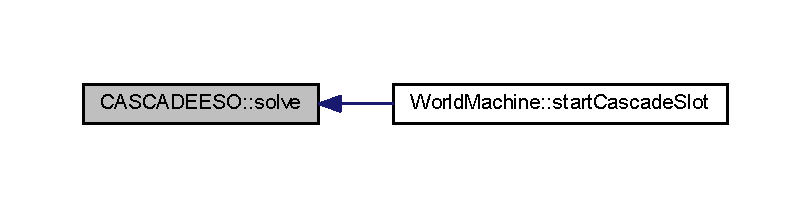
\includegraphics[width=350pt]{class_c_a_s_c_a_d_e_e_s_o_a87ddbb1f74cbb26db6dafa7d780ed7e9_icgraph}
\end{center}
\end{figure}


The documentation for this class was generated from the following file\+:\begin{DoxyCompactItemize}
\item 
\mbox{\hyperlink{cascade_8h}{cascade.\+h}}\end{DoxyCompactItemize}

\hypertarget{class_flash}{}\section{Flash$<$ TS, NP, NS, TP $>$ Class Template Reference}
\label{class_flash}\index{Flash$<$ T\+S, N\+P, N\+S, T\+P $>$@{Flash$<$ T\+S, N\+P, N\+S, T\+P $>$}}


Flashmodul.  




{\ttfamily \#include $<$flash.\+h$>$}



Inheritance diagram for Flash$<$ TS, NP, NS, TP $>$\+:
\nopagebreak
\begin{figure}[H]
\begin{center}
\leavevmode
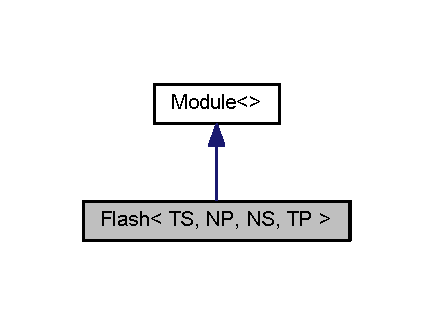
\includegraphics[width=208pt]{class_flash__inherit__graph}
\end{center}
\end{figure}


Collaboration diagram for Flash$<$ TS, NP, NS, TP $>$\+:
\nopagebreak
\begin{figure}[H]
\begin{center}
\leavevmode
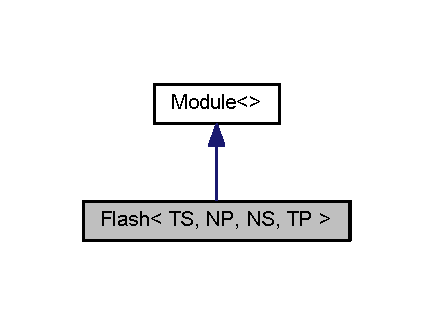
\includegraphics[width=208pt]{class_flash__coll__graph}
\end{center}
\end{figure}
\subsection*{Public Member Functions}
\begin{DoxyCompactItemize}
\item 
\mbox{\hyperlink{class_flash_afe08d3b05a9b5abe02071065b46abf62}{Flash}} (int num\+Substances, Matrix$<$ TS, Dynamic, 7 $>$ a)
\begin{DoxyCompactList}\small\item\em Konstruktor. \end{DoxyCompactList}\item 
double \& \mbox{\hyperlink{class_flash_ac3cec3cdb03bd71e7b32d7e77a209308}{pg}} ()
\begin{DoxyCompactList}\small\item\em Zugriff auf pg (Druck im \mbox{\hyperlink{class_flash}{Flash}}) \end{DoxyCompactList}\item 
double \& \mbox{\hyperlink{class_flash_ac44eff7052e26a0075c21b4f068e162e}{F}} ()
\begin{DoxyCompactList}\small\item\em Zuriff auf F (Flüssiger Zustrom) \end{DoxyCompactList}\item 
double \& \mbox{\hyperlink{class_flash_a8bfde1e00ab93b6a9b07deead0d3525a}{Lin}} ()
\item 
double \& \mbox{\hyperlink{class_flash_a74418fb8dbfaf3f5e8f99d53393f6419}{Lout}} ()
\item 
double \& \mbox{\hyperlink{class_flash_aa4358ff3c66c1c461a2dba41436b95fe}{Vin}} ()
\item 
double \& \mbox{\hyperlink{class_flash_a14aa681b115b9ca955ab775ff5e674e0}{Vout}} ()
\item 
double \& \mbox{\hyperlink{class_flash_af0f7e7c438368d98a6ea330d40b39cd3}{T}} ()
\item 
double \& \mbox{\hyperlink{class_flash_ade19a84735d622bd8fcc10bc37ed5cdd}{xini}} (int i)
\item 
double \& \mbox{\hyperlink{class_flash_a5bebef2024531af739160f0fc23e3086}{yini}} (int i)
\item 
double \& \mbox{\hyperlink{class_flash_a289586a8a31a503bd4f96ea9455f235e}{xi}} (int i)
\item 
double \& \mbox{\hyperlink{class_flash_a2af985b9562aa54cbc5c3dfd2f4292ef}{yi}} (int i)
\item 
double \& \mbox{\hyperlink{class_flash_a5ae7d29d13281fafa84cc9c247461fda}{ki}} (int i)
\item 
double \& \mbox{\hyperlink{class_flash_ae54dbc3d5d7b87c854a765e9b5f4e519}{pi}} (int i)
\item 
V\+TS \mbox{\hyperlink{class_flash_ad29e755877ca96aa5b9f34a10d6cd8b2}{f}} ()
\begin{DoxyCompactList}\small\item\em f ; muss gleich null sein um das N\+LS zu lösen (aus Aufgabenstellung) \end{DoxyCompactList}\item 
M\+TS \mbox{\hyperlink{class_flash_a83e35b3ab13b3705f0fe06c40b800a8b}{dfdx}} ()
\begin{DoxyCompactList}\small\item\em dfdx ; für den Newton-\/\+Löser \end{DoxyCompactList}\end{DoxyCompactItemize}
\subsection*{Additional Inherited Members}


\subsection{Detailed Description}
\subsubsection*{template$<$typename TS = double, int NP = Dynamic, int NS = Dynamic, typename TP = TS$>$\newline
class Flash$<$ T\+S, N\+P, N\+S, T\+P $>$}

Flashmodul. 

Ein spezifisches Bauteil. Es handelt sich um einen \mbox{\hyperlink{class_flash}{Flash}}, einen einstufigen Entspannungsverdampfer.

Besitzt durch \mbox{\hyperlink{class_module}{Module}} die Eigenschaften eines N\+LS 

\subsection{Constructor \& Destructor Documentation}
\mbox{\Hypertarget{class_flash_afe08d3b05a9b5abe02071065b46abf62}\label{class_flash_afe08d3b05a9b5abe02071065b46abf62}} 
\index{Flash@{Flash}!Flash@{Flash}}
\index{Flash@{Flash}!Flash@{Flash}}
\subsubsection{\texorpdfstring{Flash()}{Flash()}}
{\footnotesize\ttfamily template$<$typename TS = double, int NP = Dynamic, int NS = Dynamic, typename TP = TS$>$ \\
\mbox{\hyperlink{class_flash}{Flash}}$<$ TS, NP, NS, TP $>$\+::\mbox{\hyperlink{class_flash}{Flash}} (\begin{DoxyParamCaption}\item[{int}]{num\+Substances,  }\item[{Matrix$<$ TS, Dynamic, 7 $>$}]{a }\end{DoxyParamCaption})\hspace{0.3cm}{\ttfamily [inline]}}



Konstruktor. 


\begin{DoxyParams}{Parameters}
{\em num\+Substances} & Anzahl der verschiedenen Substanzen im Gemisch \\
\hline
{\em a} & Antoine-\/\+Parameter für die Substanzen (num\+Substances$\ast$7 Matrix) \\
\hline
\end{DoxyParams}
\+\_\+x\+: Lin, Lout, Vin, Vout, T, xini, yini, xi..., yi..., ki..., pi...

\subsection{Member Function Documentation}
\mbox{\Hypertarget{class_flash_a83e35b3ab13b3705f0fe06c40b800a8b}\label{class_flash_a83e35b3ab13b3705f0fe06c40b800a8b}} 
\index{Flash@{Flash}!dfdx@{dfdx}}
\index{dfdx@{dfdx}!Flash@{Flash}}
\subsubsection{\texorpdfstring{dfdx()}{dfdx()}}
{\footnotesize\ttfamily template$<$typename TS = double, int NP = Dynamic, int NS = Dynamic, typename TP = TS$>$ \\
M\+TS \mbox{\hyperlink{class_flash}{Flash}}$<$ TS, NP, NS, TP $>$\+::dfdx (\begin{DoxyParamCaption}{ }\end{DoxyParamCaption})\hspace{0.3cm}{\ttfamily [inline]}, {\ttfamily [virtual]}}



dfdx ; für den Newton-\/\+Löser 

\begin{DoxyReturn}{Returns}
dfdx in Abhängigkeit der Variablen 
\end{DoxyReturn}


Implements \mbox{\hyperlink{class_module_a0762d7cbad2a73d5eff3f2f1155e8e33}{Module$<$$>$}}.

Here is the call graph for this function\+:
\nopagebreak
\begin{figure}[H]
\begin{center}
\leavevmode
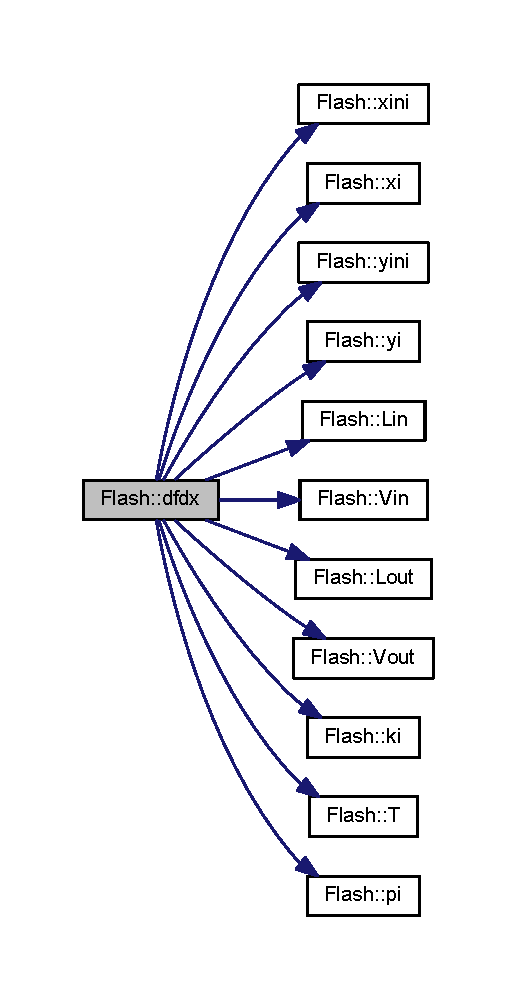
\includegraphics[width=248pt]{class_flash_a83e35b3ab13b3705f0fe06c40b800a8b_cgraph}
\end{center}
\end{figure}
\mbox{\Hypertarget{class_flash_ac44eff7052e26a0075c21b4f068e162e}\label{class_flash_ac44eff7052e26a0075c21b4f068e162e}} 
\index{Flash@{Flash}!F@{F}}
\index{F@{F}!Flash@{Flash}}
\subsubsection{\texorpdfstring{F()}{F()}}
{\footnotesize\ttfamily template$<$typename TS = double, int NP = Dynamic, int NS = Dynamic, typename TP = TS$>$ \\
double\& \mbox{\hyperlink{class_flash}{Flash}}$<$ TS, NP, NS, TP $>$\+::F (\begin{DoxyParamCaption}{ }\end{DoxyParamCaption})\hspace{0.3cm}{\ttfamily [inline]}}



Zuriff auf F (Flüssiger Zustrom) 

\begin{DoxyReturn}{Returns}
\+\_\+F 
\end{DoxyReturn}
Here is the caller graph for this function\+:
\nopagebreak
\begin{figure}[H]
\begin{center}
\leavevmode
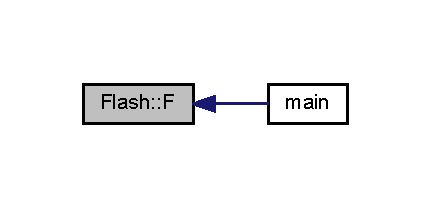
\includegraphics[width=207pt]{class_flash_ac44eff7052e26a0075c21b4f068e162e_icgraph}
\end{center}
\end{figure}
\mbox{\Hypertarget{class_flash_ad29e755877ca96aa5b9f34a10d6cd8b2}\label{class_flash_ad29e755877ca96aa5b9f34a10d6cd8b2}} 
\index{Flash@{Flash}!f@{f}}
\index{f@{f}!Flash@{Flash}}
\subsubsection{\texorpdfstring{f()}{f()}}
{\footnotesize\ttfamily template$<$typename TS = double, int NP = Dynamic, int NS = Dynamic, typename TP = TS$>$ \\
V\+TS \mbox{\hyperlink{class_flash}{Flash}}$<$ TS, NP, NS, TP $>$\+::f (\begin{DoxyParamCaption}{ }\end{DoxyParamCaption})\hspace{0.3cm}{\ttfamily [inline]}, {\ttfamily [virtual]}}



f ; muss gleich null sein um das N\+LS zu lösen (aus Aufgabenstellung) 

\begin{DoxyReturn}{Returns}
f in Abhängigkeit der Variablen 
\end{DoxyReturn}


Implements \mbox{\hyperlink{class_module_a2499211a4fc52bc33512761ea7fb3c62}{Module$<$$>$}}.

Here is the call graph for this function\+:
\nopagebreak
\begin{figure}[H]
\begin{center}
\leavevmode
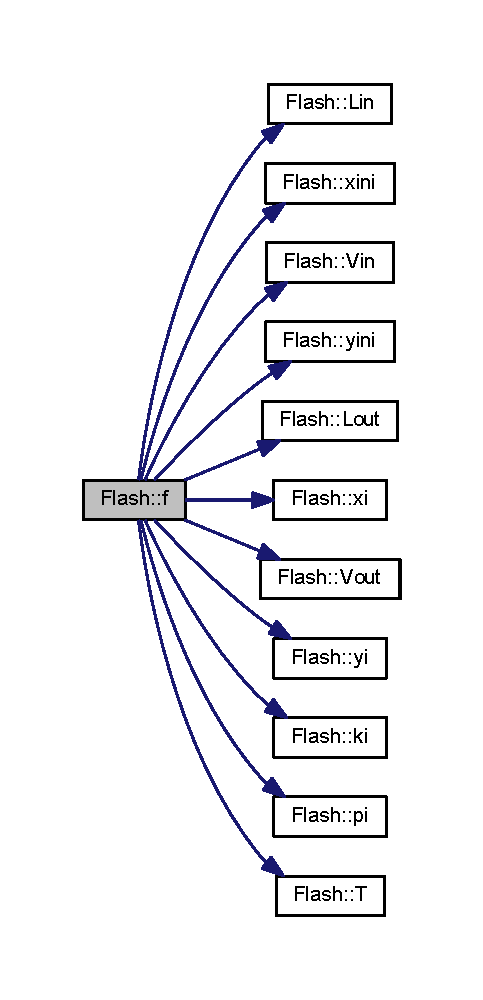
\includegraphics[width=232pt]{class_flash_ad29e755877ca96aa5b9f34a10d6cd8b2_cgraph}
\end{center}
\end{figure}
Here is the caller graph for this function\+:
\nopagebreak
\begin{figure}[H]
\begin{center}
\leavevmode
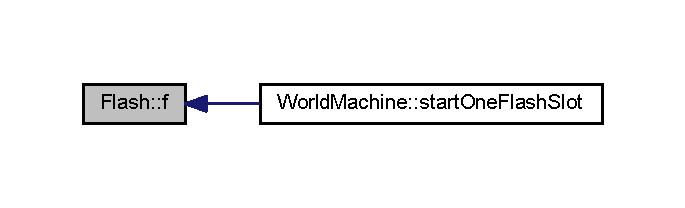
\includegraphics[width=203pt]{class_flash_ad29e755877ca96aa5b9f34a10d6cd8b2_icgraph}
\end{center}
\end{figure}
\mbox{\Hypertarget{class_flash_a5ae7d29d13281fafa84cc9c247461fda}\label{class_flash_a5ae7d29d13281fafa84cc9c247461fda}} 
\index{Flash@{Flash}!ki@{ki}}
\index{ki@{ki}!Flash@{Flash}}
\subsubsection{\texorpdfstring{ki()}{ki()}}
{\footnotesize\ttfamily template$<$typename TS = double, int NP = Dynamic, int NS = Dynamic, typename TP = TS$>$ \\
double\& \mbox{\hyperlink{class_flash}{Flash}}$<$ TS, NP, NS, TP $>$\+::ki (\begin{DoxyParamCaption}\item[{int}]{i }\end{DoxyParamCaption})\hspace{0.3cm}{\ttfamily [inline]}}

Here is the caller graph for this function\+:
\nopagebreak
\begin{figure}[H]
\begin{center}
\leavevmode
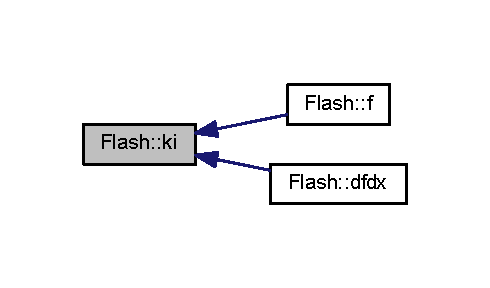
\includegraphics[width=309pt]{class_flash_a5ae7d29d13281fafa84cc9c247461fda_icgraph}
\end{center}
\end{figure}
\mbox{\Hypertarget{class_flash_a8bfde1e00ab93b6a9b07deead0d3525a}\label{class_flash_a8bfde1e00ab93b6a9b07deead0d3525a}} 
\index{Flash@{Flash}!Lin@{Lin}}
\index{Lin@{Lin}!Flash@{Flash}}
\subsubsection{\texorpdfstring{Lin()}{Lin()}}
{\footnotesize\ttfamily template$<$typename TS = double, int NP = Dynamic, int NS = Dynamic, typename TP = TS$>$ \\
double\& \mbox{\hyperlink{class_flash}{Flash}}$<$ TS, NP, NS, TP $>$\+::Lin (\begin{DoxyParamCaption}{ }\end{DoxyParamCaption})\hspace{0.3cm}{\ttfamily [inline]}}

Here is the caller graph for this function\+:
\nopagebreak
\begin{figure}[H]
\begin{center}
\leavevmode
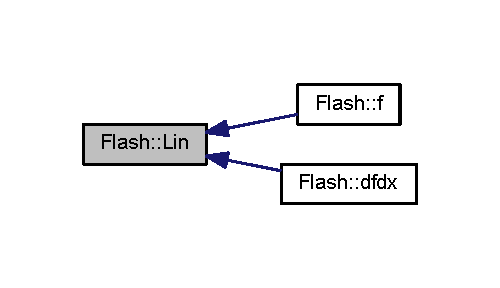
\includegraphics[width=314pt]{class_flash_a8bfde1e00ab93b6a9b07deead0d3525a_icgraph}
\end{center}
\end{figure}
\mbox{\Hypertarget{class_flash_a74418fb8dbfaf3f5e8f99d53393f6419}\label{class_flash_a74418fb8dbfaf3f5e8f99d53393f6419}} 
\index{Flash@{Flash}!Lout@{Lout}}
\index{Lout@{Lout}!Flash@{Flash}}
\subsubsection{\texorpdfstring{Lout()}{Lout()}}
{\footnotesize\ttfamily template$<$typename TS = double, int NP = Dynamic, int NS = Dynamic, typename TP = TS$>$ \\
double\& \mbox{\hyperlink{class_flash}{Flash}}$<$ TS, NP, NS, TP $>$\+::Lout (\begin{DoxyParamCaption}{ }\end{DoxyParamCaption})\hspace{0.3cm}{\ttfamily [inline]}}

Here is the caller graph for this function\+:
\nopagebreak
\begin{figure}[H]
\begin{center}
\leavevmode
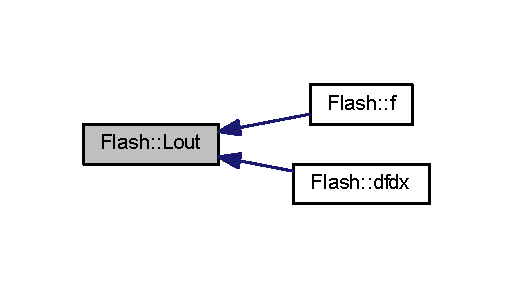
\includegraphics[width=320pt]{class_flash_a74418fb8dbfaf3f5e8f99d53393f6419_icgraph}
\end{center}
\end{figure}
\mbox{\Hypertarget{class_flash_ac3cec3cdb03bd71e7b32d7e77a209308}\label{class_flash_ac3cec3cdb03bd71e7b32d7e77a209308}} 
\index{Flash@{Flash}!pg@{pg}}
\index{pg@{pg}!Flash@{Flash}}
\subsubsection{\texorpdfstring{pg()}{pg()}}
{\footnotesize\ttfamily template$<$typename TS = double, int NP = Dynamic, int NS = Dynamic, typename TP = TS$>$ \\
double\& \mbox{\hyperlink{class_flash}{Flash}}$<$ TS, NP, NS, TP $>$\+::pg (\begin{DoxyParamCaption}{ }\end{DoxyParamCaption})\hspace{0.3cm}{\ttfamily [inline]}}



Zugriff auf pg (Druck im \mbox{\hyperlink{class_flash}{Flash}}) 

\begin{DoxyReturn}{Returns}
\+\_\+pg 
\end{DoxyReturn}
Here is the caller graph for this function\+:
\nopagebreak
\begin{figure}[H]
\begin{center}
\leavevmode
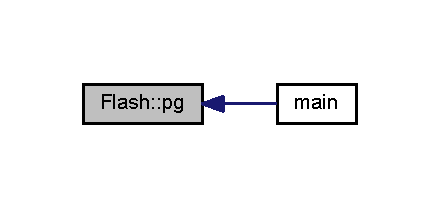
\includegraphics[width=211pt]{class_flash_ac3cec3cdb03bd71e7b32d7e77a209308_icgraph}
\end{center}
\end{figure}
\mbox{\Hypertarget{class_flash_ae54dbc3d5d7b87c854a765e9b5f4e519}\label{class_flash_ae54dbc3d5d7b87c854a765e9b5f4e519}} 
\index{Flash@{Flash}!pi@{pi}}
\index{pi@{pi}!Flash@{Flash}}
\subsubsection{\texorpdfstring{pi()}{pi()}}
{\footnotesize\ttfamily template$<$typename TS = double, int NP = Dynamic, int NS = Dynamic, typename TP = TS$>$ \\
double\& \mbox{\hyperlink{class_flash}{Flash}}$<$ TS, NP, NS, TP $>$\+::pi (\begin{DoxyParamCaption}\item[{int}]{i }\end{DoxyParamCaption})\hspace{0.3cm}{\ttfamily [inline]}}

Here is the caller graph for this function\+:
\nopagebreak
\begin{figure}[H]
\begin{center}
\leavevmode
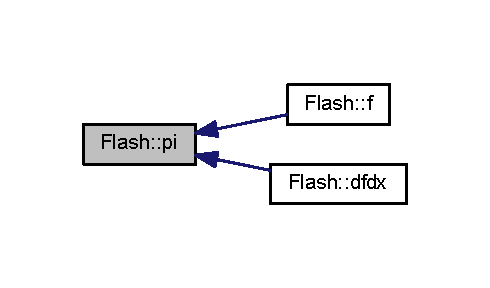
\includegraphics[width=309pt]{class_flash_ae54dbc3d5d7b87c854a765e9b5f4e519_icgraph}
\end{center}
\end{figure}
\mbox{\Hypertarget{class_flash_af0f7e7c438368d98a6ea330d40b39cd3}\label{class_flash_af0f7e7c438368d98a6ea330d40b39cd3}} 
\index{Flash@{Flash}!T@{T}}
\index{T@{T}!Flash@{Flash}}
\subsubsection{\texorpdfstring{T()}{T()}}
{\footnotesize\ttfamily template$<$typename TS = double, int NP = Dynamic, int NS = Dynamic, typename TP = TS$>$ \\
double\& \mbox{\hyperlink{class_flash}{Flash}}$<$ TS, NP, NS, TP $>$\+::T (\begin{DoxyParamCaption}{ }\end{DoxyParamCaption})\hspace{0.3cm}{\ttfamily [inline]}}

Here is the caller graph for this function\+:
\nopagebreak
\begin{figure}[H]
\begin{center}
\leavevmode
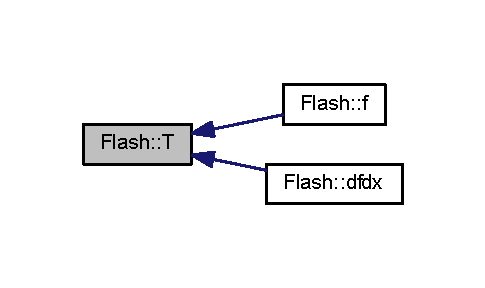
\includegraphics[width=307pt]{class_flash_af0f7e7c438368d98a6ea330d40b39cd3_icgraph}
\end{center}
\end{figure}
\mbox{\Hypertarget{class_flash_aa4358ff3c66c1c461a2dba41436b95fe}\label{class_flash_aa4358ff3c66c1c461a2dba41436b95fe}} 
\index{Flash@{Flash}!Vin@{Vin}}
\index{Vin@{Vin}!Flash@{Flash}}
\subsubsection{\texorpdfstring{Vin()}{Vin()}}
{\footnotesize\ttfamily template$<$typename TS = double, int NP = Dynamic, int NS = Dynamic, typename TP = TS$>$ \\
double\& \mbox{\hyperlink{class_flash}{Flash}}$<$ TS, NP, NS, TP $>$\+::Vin (\begin{DoxyParamCaption}{ }\end{DoxyParamCaption})\hspace{0.3cm}{\ttfamily [inline]}}

Here is the caller graph for this function\+:
\nopagebreak
\begin{figure}[H]
\begin{center}
\leavevmode
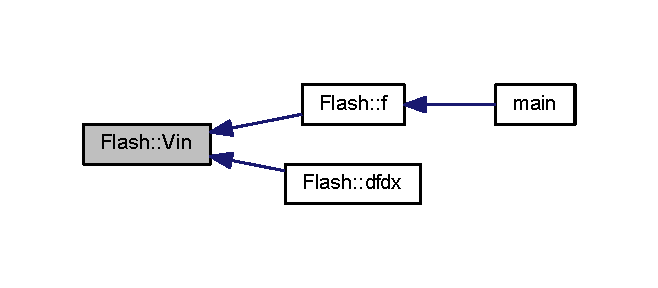
\includegraphics[width=316pt]{class_flash_aa4358ff3c66c1c461a2dba41436b95fe_icgraph}
\end{center}
\end{figure}
\mbox{\Hypertarget{class_flash_a14aa681b115b9ca955ab775ff5e674e0}\label{class_flash_a14aa681b115b9ca955ab775ff5e674e0}} 
\index{Flash@{Flash}!Vout@{Vout}}
\index{Vout@{Vout}!Flash@{Flash}}
\subsubsection{\texorpdfstring{Vout()}{Vout()}}
{\footnotesize\ttfamily template$<$typename TS = double, int NP = Dynamic, int NS = Dynamic, typename TP = TS$>$ \\
double\& \mbox{\hyperlink{class_flash}{Flash}}$<$ TS, NP, NS, TP $>$\+::Vout (\begin{DoxyParamCaption}{ }\end{DoxyParamCaption})\hspace{0.3cm}{\ttfamily [inline]}}

Here is the caller graph for this function\+:
\nopagebreak
\begin{figure}[H]
\begin{center}
\leavevmode
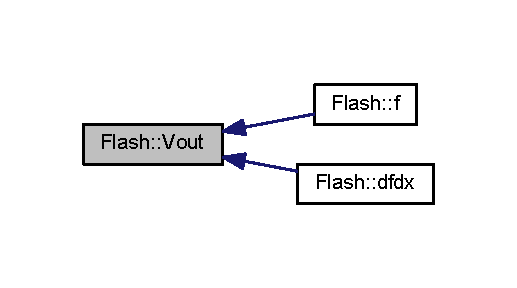
\includegraphics[width=322pt]{class_flash_a14aa681b115b9ca955ab775ff5e674e0_icgraph}
\end{center}
\end{figure}
\mbox{\Hypertarget{class_flash_a289586a8a31a503bd4f96ea9455f235e}\label{class_flash_a289586a8a31a503bd4f96ea9455f235e}} 
\index{Flash@{Flash}!xi@{xi}}
\index{xi@{xi}!Flash@{Flash}}
\subsubsection{\texorpdfstring{xi()}{xi()}}
{\footnotesize\ttfamily template$<$typename TS = double, int NP = Dynamic, int NS = Dynamic, typename TP = TS$>$ \\
double\& \mbox{\hyperlink{class_flash}{Flash}}$<$ TS, NP, NS, TP $>$\+::xi (\begin{DoxyParamCaption}\item[{int}]{i }\end{DoxyParamCaption})\hspace{0.3cm}{\ttfamily [inline]}}

Here is the caller graph for this function\+:
\nopagebreak
\begin{figure}[H]
\begin{center}
\leavevmode
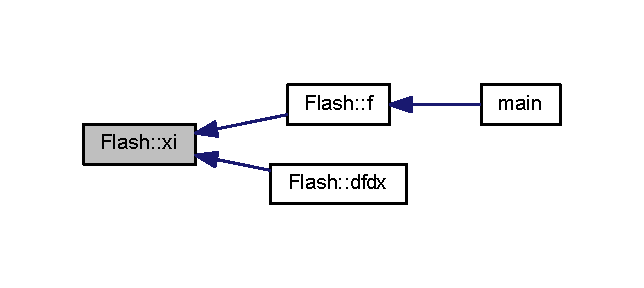
\includegraphics[width=309pt]{class_flash_a289586a8a31a503bd4f96ea9455f235e_icgraph}
\end{center}
\end{figure}
\mbox{\Hypertarget{class_flash_ade19a84735d622bd8fcc10bc37ed5cdd}\label{class_flash_ade19a84735d622bd8fcc10bc37ed5cdd}} 
\index{Flash@{Flash}!xini@{xini}}
\index{xini@{xini}!Flash@{Flash}}
\subsubsection{\texorpdfstring{xini()}{xini()}}
{\footnotesize\ttfamily template$<$typename TS = double, int NP = Dynamic, int NS = Dynamic, typename TP = TS$>$ \\
double\& \mbox{\hyperlink{class_flash}{Flash}}$<$ TS, NP, NS, TP $>$\+::xini (\begin{DoxyParamCaption}\item[{int}]{i }\end{DoxyParamCaption})\hspace{0.3cm}{\ttfamily [inline]}}

Here is the caller graph for this function\+:
\nopagebreak
\begin{figure}[H]
\begin{center}
\leavevmode
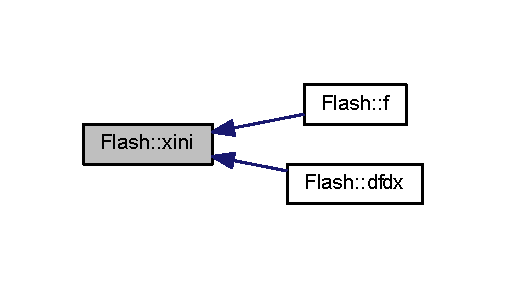
\includegraphics[width=317pt]{class_flash_ade19a84735d622bd8fcc10bc37ed5cdd_icgraph}
\end{center}
\end{figure}
\mbox{\Hypertarget{class_flash_a2af985b9562aa54cbc5c3dfd2f4292ef}\label{class_flash_a2af985b9562aa54cbc5c3dfd2f4292ef}} 
\index{Flash@{Flash}!yi@{yi}}
\index{yi@{yi}!Flash@{Flash}}
\subsubsection{\texorpdfstring{yi()}{yi()}}
{\footnotesize\ttfamily template$<$typename TS = double, int NP = Dynamic, int NS = Dynamic, typename TP = TS$>$ \\
double\& \mbox{\hyperlink{class_flash}{Flash}}$<$ TS, NP, NS, TP $>$\+::yi (\begin{DoxyParamCaption}\item[{int}]{i }\end{DoxyParamCaption})\hspace{0.3cm}{\ttfamily [inline]}}

Here is the caller graph for this function\+:
\nopagebreak
\begin{figure}[H]
\begin{center}
\leavevmode
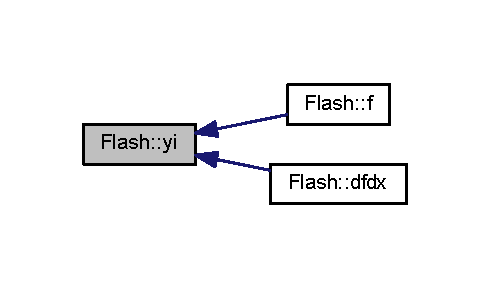
\includegraphics[width=309pt]{class_flash_a2af985b9562aa54cbc5c3dfd2f4292ef_icgraph}
\end{center}
\end{figure}
\mbox{\Hypertarget{class_flash_a5bebef2024531af739160f0fc23e3086}\label{class_flash_a5bebef2024531af739160f0fc23e3086}} 
\index{Flash@{Flash}!yini@{yini}}
\index{yini@{yini}!Flash@{Flash}}
\subsubsection{\texorpdfstring{yini()}{yini()}}
{\footnotesize\ttfamily template$<$typename TS = double, int NP = Dynamic, int NS = Dynamic, typename TP = TS$>$ \\
double\& \mbox{\hyperlink{class_flash}{Flash}}$<$ TS, NP, NS, TP $>$\+::yini (\begin{DoxyParamCaption}\item[{int}]{i }\end{DoxyParamCaption})\hspace{0.3cm}{\ttfamily [inline]}}

Here is the caller graph for this function\+:
\nopagebreak
\begin{figure}[H]
\begin{center}
\leavevmode
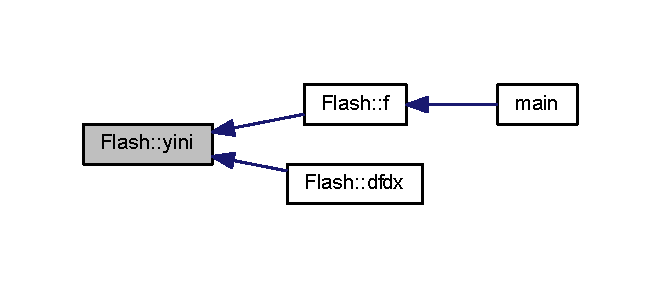
\includegraphics[width=317pt]{class_flash_a5bebef2024531af739160f0fc23e3086_icgraph}
\end{center}
\end{figure}


The documentation for this class was generated from the following file\+:\begin{DoxyCompactItemize}
\item 
\mbox{\hyperlink{flash_8h}{flash.\+h}}\end{DoxyCompactItemize}

\hypertarget{class_l_i_n_e_a_r___s_o_l_v_e_r}{}\section{L\+I\+N\+E\+A\+R\+\_\+\+S\+O\+L\+V\+ER$<$ TA, N, Tb, Tx $>$ Class Template Reference}
\label{class_l_i_n_e_a_r___s_o_l_v_e_r}\index{L\+I\+N\+E\+A\+R\+\_\+\+S\+O\+L\+V\+E\+R$<$ T\+A, N, Tb, Tx $>$@{L\+I\+N\+E\+A\+R\+\_\+\+S\+O\+L\+V\+E\+R$<$ T\+A, N, Tb, Tx $>$}}


{\ttfamily \#include $<$lin\+\_\+sys.\+h$>$}



Inheritance diagram for L\+I\+N\+E\+A\+R\+\_\+\+S\+O\+L\+V\+ER$<$ TA, N, Tb, Tx $>$\+:
\nopagebreak
\begin{figure}[H]
\begin{center}
\leavevmode
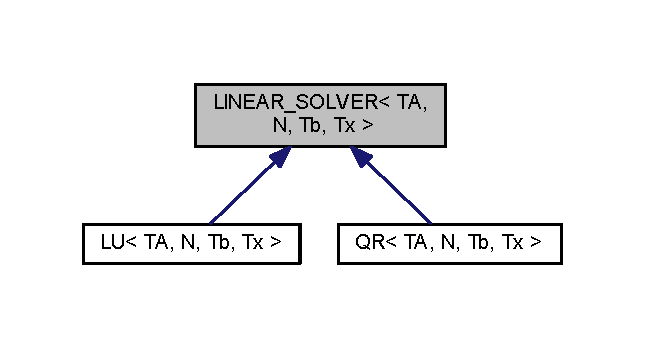
\includegraphics[width=310pt]{class_l_i_n_e_a_r___s_o_l_v_e_r__inherit__graph}
\end{center}
\end{figure}
\subsection*{Public Member Functions}
\begin{DoxyCompactItemize}
\item 
virtual void \mbox{\hyperlink{class_l_i_n_e_a_r___s_o_l_v_e_r_a83c4d3b280e57814ec091dd9f8927c24}{solve}} (\mbox{\hyperlink{class_l_i_n_e_a_r___s_y_s_t_e_m}{L\+I\+N\+E\+A\+R\+\_\+\+S\+Y\+S\+T\+EM}}$<$ TA, N, Tb, Tx $>$ \&)=0
\end{DoxyCompactItemize}


\subsection{Member Function Documentation}
\mbox{\Hypertarget{class_l_i_n_e_a_r___s_o_l_v_e_r_a83c4d3b280e57814ec091dd9f8927c24}\label{class_l_i_n_e_a_r___s_o_l_v_e_r_a83c4d3b280e57814ec091dd9f8927c24}} 
\index{L\+I\+N\+E\+A\+R\+\_\+\+S\+O\+L\+V\+ER@{L\+I\+N\+E\+A\+R\+\_\+\+S\+O\+L\+V\+ER}!solve@{solve}}
\index{solve@{solve}!L\+I\+N\+E\+A\+R\+\_\+\+S\+O\+L\+V\+ER@{L\+I\+N\+E\+A\+R\+\_\+\+S\+O\+L\+V\+ER}}
\subsubsection{\texorpdfstring{solve()}{solve()}}
{\footnotesize\ttfamily template$<$typename TA = double, int N = Dynamic, typename Tb = TA, typename Tx = Tb$>$ \\
virtual void \mbox{\hyperlink{class_l_i_n_e_a_r___s_o_l_v_e_r}{L\+I\+N\+E\+A\+R\+\_\+\+S\+O\+L\+V\+ER}}$<$ TA, N, Tb, Tx $>$\+::solve (\begin{DoxyParamCaption}\item[{\mbox{\hyperlink{class_l_i_n_e_a_r___s_y_s_t_e_m}{L\+I\+N\+E\+A\+R\+\_\+\+S\+Y\+S\+T\+EM}}$<$ TA, N, Tb, Tx $>$ \&}]{ }\end{DoxyParamCaption})\hspace{0.3cm}{\ttfamily [pure virtual]}}



Implemented in \mbox{\hyperlink{class_q_r_ab8f49cec36214bdcd9fca78e89c3737e}{Q\+R$<$ T\+A, N, Tb, Tx $>$}}, and \mbox{\hyperlink{class_l_u_a624d7ff38645debae206313534516f49}{L\+U$<$ T\+A, N, Tb, Tx $>$}}.

Here is the caller graph for this function\+:
\nopagebreak
\begin{figure}[H]
\begin{center}
\leavevmode
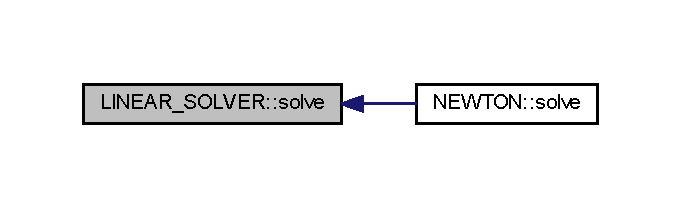
\includegraphics[width=327pt]{class_l_i_n_e_a_r___s_o_l_v_e_r_a83c4d3b280e57814ec091dd9f8927c24_icgraph}
\end{center}
\end{figure}


The documentation for this class was generated from the following file\+:\begin{DoxyCompactItemize}
\item 
\mbox{\hyperlink{lin__sys_8h}{lin\+\_\+sys.\+h}}\end{DoxyCompactItemize}

\hypertarget{class_l_i_n_e_a_r___s_y_s_t_e_m}{}\section{L\+I\+N\+E\+A\+R\+\_\+\+S\+Y\+S\+T\+EM$<$ TA, N, Tb, Tx $>$ Class Template Reference}
\label{class_l_i_n_e_a_r___s_y_s_t_e_m}\index{L\+I\+N\+E\+A\+R\+\_\+\+S\+Y\+S\+T\+E\+M$<$ T\+A, N, Tb, Tx $>$@{L\+I\+N\+E\+A\+R\+\_\+\+S\+Y\+S\+T\+E\+M$<$ T\+A, N, Tb, Tx $>$}}


{\ttfamily \#include $<$lin\+\_\+sys.\+h$>$}

\subsection*{Public Member Functions}
\begin{DoxyCompactItemize}
\item 
\mbox{\hyperlink{class_l_i_n_e_a_r___s_y_s_t_e_m_a7486740300aa9998e1aa4f9d90790eb2}{L\+I\+N\+E\+A\+R\+\_\+\+S\+Y\+S\+T\+EM}} (const int \&n)
\item 
V\+Tx \& \mbox{\hyperlink{class_l_i_n_e_a_r___s_y_s_t_e_m_a0585adb67fae39d29e887d03d071fc74}{x}} ()
\item 
Tx \& \mbox{\hyperlink{class_l_i_n_e_a_r___s_y_s_t_e_m_ad00a0cae1d479dd527cc374c210b9429}{x}} (int i)
\item 
V\+Tb \& \mbox{\hyperlink{class_l_i_n_e_a_r___s_y_s_t_e_m_a6754b4aaf5db40c45522d289e969f917}{b}} ()
\item 
Tb \& \mbox{\hyperlink{class_l_i_n_e_a_r___s_y_s_t_e_m_ae7c2a505d8cd0c6eb4b49bc0ece4e233}{b}} (int i)
\item 
M\+TA \& \mbox{\hyperlink{class_l_i_n_e_a_r___s_y_s_t_e_m_a307c8896bb3218768f016a2a24de3bcd}{A}} ()
\item 
TA \& \mbox{\hyperlink{class_l_i_n_e_a_r___s_y_s_t_e_m_a5163aedcb567d591f5812bd3c892fb07}{A}} (int i, int j)
\end{DoxyCompactItemize}
\subsection*{Protected Attributes}
\begin{DoxyCompactItemize}
\item 
V\+Tx \mbox{\hyperlink{class_l_i_n_e_a_r___s_y_s_t_e_m_abc1a6ac63a5c66a14e47cdb22559fefa}{\+\_\+x}}
\item 
V\+Tb \mbox{\hyperlink{class_l_i_n_e_a_r___s_y_s_t_e_m_a2a040e59b49e900b61c4db4385623fd0}{\+\_\+b}}
\item 
M\+TA \mbox{\hyperlink{class_l_i_n_e_a_r___s_y_s_t_e_m_afee92f4a1bc570f9ead4742047756525}{\+\_\+A}}
\end{DoxyCompactItemize}


\subsection{Detailed Description}
\subsubsection*{template$<$typename TA = double, int N = Dynamic, typename Tb = TA, typename Tx = Tb$>$\newline
class L\+I\+N\+E\+A\+R\+\_\+\+S\+Y\+S\+T\+E\+M$<$ T\+A, N, Tb, Tx $>$}

Basierend auf \mbox{\hyperlink{lin__sys_8h}{lin\+\_\+sys.\+h}} von Uwe Naumann 

\subsection{Constructor \& Destructor Documentation}
\mbox{\Hypertarget{class_l_i_n_e_a_r___s_y_s_t_e_m_a7486740300aa9998e1aa4f9d90790eb2}\label{class_l_i_n_e_a_r___s_y_s_t_e_m_a7486740300aa9998e1aa4f9d90790eb2}} 
\index{L\+I\+N\+E\+A\+R\+\_\+\+S\+Y\+S\+T\+EM@{L\+I\+N\+E\+A\+R\+\_\+\+S\+Y\+S\+T\+EM}!L\+I\+N\+E\+A\+R\+\_\+\+S\+Y\+S\+T\+EM@{L\+I\+N\+E\+A\+R\+\_\+\+S\+Y\+S\+T\+EM}}
\index{L\+I\+N\+E\+A\+R\+\_\+\+S\+Y\+S\+T\+EM@{L\+I\+N\+E\+A\+R\+\_\+\+S\+Y\+S\+T\+EM}!L\+I\+N\+E\+A\+R\+\_\+\+S\+Y\+S\+T\+EM@{L\+I\+N\+E\+A\+R\+\_\+\+S\+Y\+S\+T\+EM}}
\subsubsection{\texorpdfstring{L\+I\+N\+E\+A\+R\+\_\+\+S\+Y\+S\+T\+E\+M()}{LINEAR\_SYSTEM()}}
{\footnotesize\ttfamily template$<$typename TA = double, int N = Dynamic, typename Tb = TA, typename Tx = Tb$>$ \\
\mbox{\hyperlink{class_l_i_n_e_a_r___s_y_s_t_e_m}{L\+I\+N\+E\+A\+R\+\_\+\+S\+Y\+S\+T\+EM}}$<$ TA, N, Tb, Tx $>$\+::\mbox{\hyperlink{class_l_i_n_e_a_r___s_y_s_t_e_m}{L\+I\+N\+E\+A\+R\+\_\+\+S\+Y\+S\+T\+EM}} (\begin{DoxyParamCaption}\item[{const int \&}]{n }\end{DoxyParamCaption})\hspace{0.3cm}{\ttfamily [inline]}}



\subsection{Member Function Documentation}
\mbox{\Hypertarget{class_l_i_n_e_a_r___s_y_s_t_e_m_a307c8896bb3218768f016a2a24de3bcd}\label{class_l_i_n_e_a_r___s_y_s_t_e_m_a307c8896bb3218768f016a2a24de3bcd}} 
\index{L\+I\+N\+E\+A\+R\+\_\+\+S\+Y\+S\+T\+EM@{L\+I\+N\+E\+A\+R\+\_\+\+S\+Y\+S\+T\+EM}!A@{A}}
\index{A@{A}!L\+I\+N\+E\+A\+R\+\_\+\+S\+Y\+S\+T\+EM@{L\+I\+N\+E\+A\+R\+\_\+\+S\+Y\+S\+T\+EM}}
\subsubsection{\texorpdfstring{A()}{A()}\hspace{0.1cm}{\footnotesize\ttfamily [1/2]}}
{\footnotesize\ttfamily template$<$typename TA = double, int N = Dynamic, typename Tb = TA, typename Tx = Tb$>$ \\
M\+TA\& \mbox{\hyperlink{class_l_i_n_e_a_r___s_y_s_t_e_m}{L\+I\+N\+E\+A\+R\+\_\+\+S\+Y\+S\+T\+EM}}$<$ TA, N, Tb, Tx $>$\+::A (\begin{DoxyParamCaption}{ }\end{DoxyParamCaption})\hspace{0.3cm}{\ttfamily [inline]}}

Here is the caller graph for this function\+:
\nopagebreak
\begin{figure}[H]
\begin{center}
\leavevmode
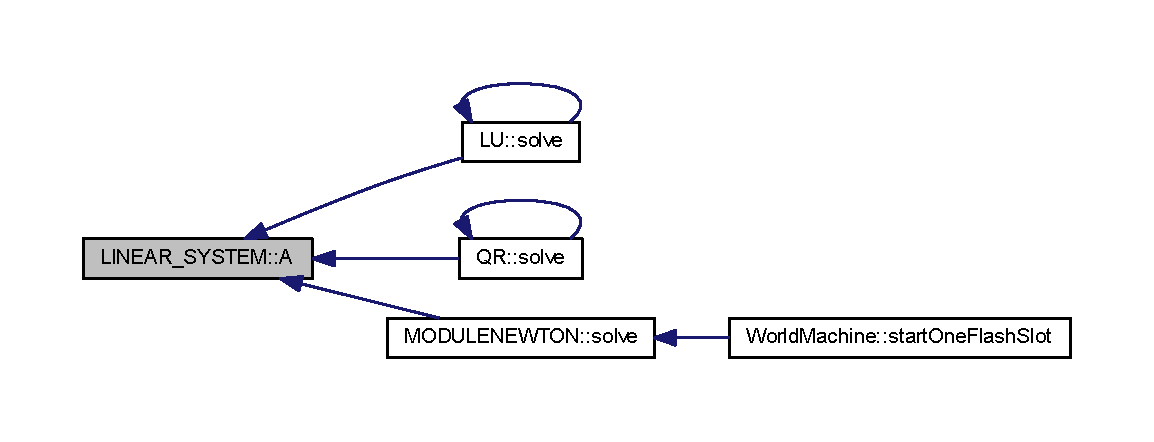
\includegraphics[width=313pt]{class_l_i_n_e_a_r___s_y_s_t_e_m_a307c8896bb3218768f016a2a24de3bcd_icgraph}
\end{center}
\end{figure}
\mbox{\Hypertarget{class_l_i_n_e_a_r___s_y_s_t_e_m_a5163aedcb567d591f5812bd3c892fb07}\label{class_l_i_n_e_a_r___s_y_s_t_e_m_a5163aedcb567d591f5812bd3c892fb07}} 
\index{L\+I\+N\+E\+A\+R\+\_\+\+S\+Y\+S\+T\+EM@{L\+I\+N\+E\+A\+R\+\_\+\+S\+Y\+S\+T\+EM}!A@{A}}
\index{A@{A}!L\+I\+N\+E\+A\+R\+\_\+\+S\+Y\+S\+T\+EM@{L\+I\+N\+E\+A\+R\+\_\+\+S\+Y\+S\+T\+EM}}
\subsubsection{\texorpdfstring{A()}{A()}\hspace{0.1cm}{\footnotesize\ttfamily [2/2]}}
{\footnotesize\ttfamily template$<$typename TA = double, int N = Dynamic, typename Tb = TA, typename Tx = Tb$>$ \\
TA\& \mbox{\hyperlink{class_l_i_n_e_a_r___s_y_s_t_e_m}{L\+I\+N\+E\+A\+R\+\_\+\+S\+Y\+S\+T\+EM}}$<$ TA, N, Tb, Tx $>$\+::A (\begin{DoxyParamCaption}\item[{int}]{i,  }\item[{int}]{j }\end{DoxyParamCaption})\hspace{0.3cm}{\ttfamily [inline]}}

\mbox{\Hypertarget{class_l_i_n_e_a_r___s_y_s_t_e_m_a6754b4aaf5db40c45522d289e969f917}\label{class_l_i_n_e_a_r___s_y_s_t_e_m_a6754b4aaf5db40c45522d289e969f917}} 
\index{L\+I\+N\+E\+A\+R\+\_\+\+S\+Y\+S\+T\+EM@{L\+I\+N\+E\+A\+R\+\_\+\+S\+Y\+S\+T\+EM}!b@{b}}
\index{b@{b}!L\+I\+N\+E\+A\+R\+\_\+\+S\+Y\+S\+T\+EM@{L\+I\+N\+E\+A\+R\+\_\+\+S\+Y\+S\+T\+EM}}
\subsubsection{\texorpdfstring{b()}{b()}\hspace{0.1cm}{\footnotesize\ttfamily [1/2]}}
{\footnotesize\ttfamily template$<$typename TA = double, int N = Dynamic, typename Tb = TA, typename Tx = Tb$>$ \\
V\+Tb\& \mbox{\hyperlink{class_l_i_n_e_a_r___s_y_s_t_e_m}{L\+I\+N\+E\+A\+R\+\_\+\+S\+Y\+S\+T\+EM}}$<$ TA, N, Tb, Tx $>$\+::b (\begin{DoxyParamCaption}{ }\end{DoxyParamCaption})\hspace{0.3cm}{\ttfamily [inline]}}

Here is the caller graph for this function\+:
\nopagebreak
\begin{figure}[H]
\begin{center}
\leavevmode
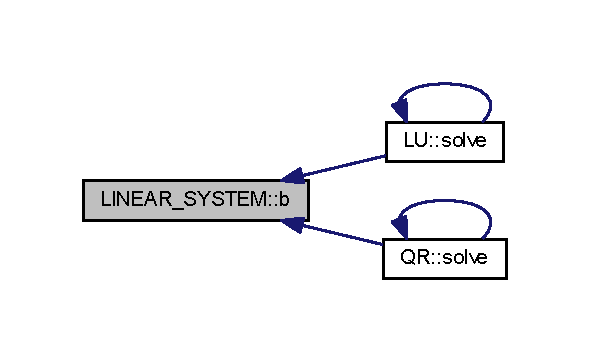
\includegraphics[width=283pt]{class_l_i_n_e_a_r___s_y_s_t_e_m_a6754b4aaf5db40c45522d289e969f917_icgraph}
\end{center}
\end{figure}
\mbox{\Hypertarget{class_l_i_n_e_a_r___s_y_s_t_e_m_ae7c2a505d8cd0c6eb4b49bc0ece4e233}\label{class_l_i_n_e_a_r___s_y_s_t_e_m_ae7c2a505d8cd0c6eb4b49bc0ece4e233}} 
\index{L\+I\+N\+E\+A\+R\+\_\+\+S\+Y\+S\+T\+EM@{L\+I\+N\+E\+A\+R\+\_\+\+S\+Y\+S\+T\+EM}!b@{b}}
\index{b@{b}!L\+I\+N\+E\+A\+R\+\_\+\+S\+Y\+S\+T\+EM@{L\+I\+N\+E\+A\+R\+\_\+\+S\+Y\+S\+T\+EM}}
\subsubsection{\texorpdfstring{b()}{b()}\hspace{0.1cm}{\footnotesize\ttfamily [2/2]}}
{\footnotesize\ttfamily template$<$typename TA = double, int N = Dynamic, typename Tb = TA, typename Tx = Tb$>$ \\
Tb\& \mbox{\hyperlink{class_l_i_n_e_a_r___s_y_s_t_e_m}{L\+I\+N\+E\+A\+R\+\_\+\+S\+Y\+S\+T\+EM}}$<$ TA, N, Tb, Tx $>$\+::b (\begin{DoxyParamCaption}\item[{int}]{i }\end{DoxyParamCaption})\hspace{0.3cm}{\ttfamily [inline]}}

\mbox{\Hypertarget{class_l_i_n_e_a_r___s_y_s_t_e_m_a0585adb67fae39d29e887d03d071fc74}\label{class_l_i_n_e_a_r___s_y_s_t_e_m_a0585adb67fae39d29e887d03d071fc74}} 
\index{L\+I\+N\+E\+A\+R\+\_\+\+S\+Y\+S\+T\+EM@{L\+I\+N\+E\+A\+R\+\_\+\+S\+Y\+S\+T\+EM}!x@{x}}
\index{x@{x}!L\+I\+N\+E\+A\+R\+\_\+\+S\+Y\+S\+T\+EM@{L\+I\+N\+E\+A\+R\+\_\+\+S\+Y\+S\+T\+EM}}
\subsubsection{\texorpdfstring{x()}{x()}\hspace{0.1cm}{\footnotesize\ttfamily [1/2]}}
{\footnotesize\ttfamily template$<$typename TA = double, int N = Dynamic, typename Tb = TA, typename Tx = Tb$>$ \\
V\+Tx\& \mbox{\hyperlink{class_l_i_n_e_a_r___s_y_s_t_e_m}{L\+I\+N\+E\+A\+R\+\_\+\+S\+Y\+S\+T\+EM}}$<$ TA, N, Tb, Tx $>$\+::x (\begin{DoxyParamCaption}{ }\end{DoxyParamCaption})\hspace{0.3cm}{\ttfamily [inline]}}

Here is the caller graph for this function\+:
\nopagebreak
\begin{figure}[H]
\begin{center}
\leavevmode
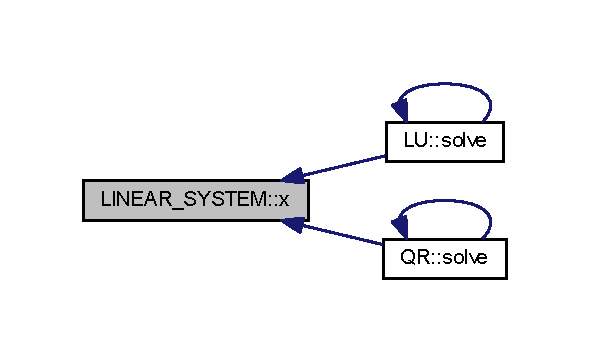
\includegraphics[width=283pt]{class_l_i_n_e_a_r___s_y_s_t_e_m_a0585adb67fae39d29e887d03d071fc74_icgraph}
\end{center}
\end{figure}
\mbox{\Hypertarget{class_l_i_n_e_a_r___s_y_s_t_e_m_ad00a0cae1d479dd527cc374c210b9429}\label{class_l_i_n_e_a_r___s_y_s_t_e_m_ad00a0cae1d479dd527cc374c210b9429}} 
\index{L\+I\+N\+E\+A\+R\+\_\+\+S\+Y\+S\+T\+EM@{L\+I\+N\+E\+A\+R\+\_\+\+S\+Y\+S\+T\+EM}!x@{x}}
\index{x@{x}!L\+I\+N\+E\+A\+R\+\_\+\+S\+Y\+S\+T\+EM@{L\+I\+N\+E\+A\+R\+\_\+\+S\+Y\+S\+T\+EM}}
\subsubsection{\texorpdfstring{x()}{x()}\hspace{0.1cm}{\footnotesize\ttfamily [2/2]}}
{\footnotesize\ttfamily template$<$typename TA = double, int N = Dynamic, typename Tb = TA, typename Tx = Tb$>$ \\
Tx\& \mbox{\hyperlink{class_l_i_n_e_a_r___s_y_s_t_e_m}{L\+I\+N\+E\+A\+R\+\_\+\+S\+Y\+S\+T\+EM}}$<$ TA, N, Tb, Tx $>$\+::x (\begin{DoxyParamCaption}\item[{int}]{i }\end{DoxyParamCaption})\hspace{0.3cm}{\ttfamily [inline]}}



\subsection{Member Data Documentation}
\mbox{\Hypertarget{class_l_i_n_e_a_r___s_y_s_t_e_m_afee92f4a1bc570f9ead4742047756525}\label{class_l_i_n_e_a_r___s_y_s_t_e_m_afee92f4a1bc570f9ead4742047756525}} 
\index{L\+I\+N\+E\+A\+R\+\_\+\+S\+Y\+S\+T\+EM@{L\+I\+N\+E\+A\+R\+\_\+\+S\+Y\+S\+T\+EM}!\+\_\+A@{\+\_\+A}}
\index{\+\_\+A@{\+\_\+A}!L\+I\+N\+E\+A\+R\+\_\+\+S\+Y\+S\+T\+EM@{L\+I\+N\+E\+A\+R\+\_\+\+S\+Y\+S\+T\+EM}}
\subsubsection{\texorpdfstring{\+\_\+A}{\_A}}
{\footnotesize\ttfamily template$<$typename TA = double, int N = Dynamic, typename Tb = TA, typename Tx = Tb$>$ \\
M\+TA \mbox{\hyperlink{class_l_i_n_e_a_r___s_y_s_t_e_m}{L\+I\+N\+E\+A\+R\+\_\+\+S\+Y\+S\+T\+EM}}$<$ TA, N, Tb, Tx $>$\+::\+\_\+A\hspace{0.3cm}{\ttfamily [protected]}}

\mbox{\Hypertarget{class_l_i_n_e_a_r___s_y_s_t_e_m_a2a040e59b49e900b61c4db4385623fd0}\label{class_l_i_n_e_a_r___s_y_s_t_e_m_a2a040e59b49e900b61c4db4385623fd0}} 
\index{L\+I\+N\+E\+A\+R\+\_\+\+S\+Y\+S\+T\+EM@{L\+I\+N\+E\+A\+R\+\_\+\+S\+Y\+S\+T\+EM}!\+\_\+b@{\+\_\+b}}
\index{\+\_\+b@{\+\_\+b}!L\+I\+N\+E\+A\+R\+\_\+\+S\+Y\+S\+T\+EM@{L\+I\+N\+E\+A\+R\+\_\+\+S\+Y\+S\+T\+EM}}
\subsubsection{\texorpdfstring{\+\_\+b}{\_b}}
{\footnotesize\ttfamily template$<$typename TA = double, int N = Dynamic, typename Tb = TA, typename Tx = Tb$>$ \\
V\+Tb \mbox{\hyperlink{class_l_i_n_e_a_r___s_y_s_t_e_m}{L\+I\+N\+E\+A\+R\+\_\+\+S\+Y\+S\+T\+EM}}$<$ TA, N, Tb, Tx $>$\+::\+\_\+b\hspace{0.3cm}{\ttfamily [protected]}}

\mbox{\Hypertarget{class_l_i_n_e_a_r___s_y_s_t_e_m_abc1a6ac63a5c66a14e47cdb22559fefa}\label{class_l_i_n_e_a_r___s_y_s_t_e_m_abc1a6ac63a5c66a14e47cdb22559fefa}} 
\index{L\+I\+N\+E\+A\+R\+\_\+\+S\+Y\+S\+T\+EM@{L\+I\+N\+E\+A\+R\+\_\+\+S\+Y\+S\+T\+EM}!\+\_\+x@{\+\_\+x}}
\index{\+\_\+x@{\+\_\+x}!L\+I\+N\+E\+A\+R\+\_\+\+S\+Y\+S\+T\+EM@{L\+I\+N\+E\+A\+R\+\_\+\+S\+Y\+S\+T\+EM}}
\subsubsection{\texorpdfstring{\+\_\+x}{\_x}}
{\footnotesize\ttfamily template$<$typename TA = double, int N = Dynamic, typename Tb = TA, typename Tx = Tb$>$ \\
V\+Tx \mbox{\hyperlink{class_l_i_n_e_a_r___s_y_s_t_e_m}{L\+I\+N\+E\+A\+R\+\_\+\+S\+Y\+S\+T\+EM}}$<$ TA, N, Tb, Tx $>$\+::\+\_\+x\hspace{0.3cm}{\ttfamily [protected]}}



The documentation for this class was generated from the following file\+:\begin{DoxyCompactItemize}
\item 
\mbox{\hyperlink{lin__sys_8h}{lin\+\_\+sys.\+h}}\end{DoxyCompactItemize}

\hypertarget{class_l_u}{}\section{LU$<$ TA, N, Tb, Tx $>$ Class Template Reference}
\label{class_l_u}\index{L\+U$<$ T\+A, N, Tb, Tx $>$@{L\+U$<$ T\+A, N, Tb, Tx $>$}}


{\ttfamily \#include $<$lin\+\_\+sys.\+h$>$}



Inheritance diagram for LU$<$ TA, N, Tb, Tx $>$\+:
\nopagebreak
\begin{figure}[H]
\begin{center}
\leavevmode
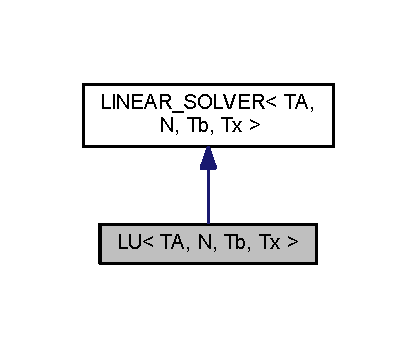
\includegraphics[width=200pt]{class_l_u__inherit__graph}
\end{center}
\end{figure}


Collaboration diagram for LU$<$ TA, N, Tb, Tx $>$\+:
\nopagebreak
\begin{figure}[H]
\begin{center}
\leavevmode
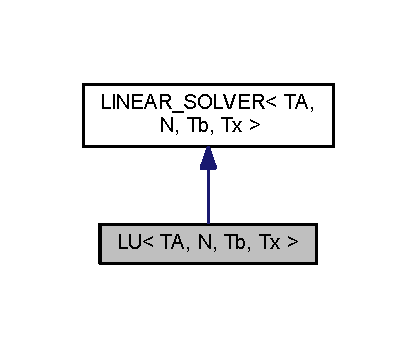
\includegraphics[width=200pt]{class_l_u__coll__graph}
\end{center}
\end{figure}
\subsection*{Public Member Functions}
\begin{DoxyCompactItemize}
\item 
void \mbox{\hyperlink{class_l_u_a624d7ff38645debae206313534516f49}{solve}} (\mbox{\hyperlink{class_l_i_n_e_a_r___s_y_s_t_e_m}{L\+I\+N\+E\+A\+R\+\_\+\+S\+Y\+S\+T\+EM}}$<$ TA, N, Tb, Tx $>$ \&s)
\end{DoxyCompactItemize}


\subsection{Member Function Documentation}
\mbox{\Hypertarget{class_l_u_a624d7ff38645debae206313534516f49}\label{class_l_u_a624d7ff38645debae206313534516f49}} 
\index{LU@{LU}!solve@{solve}}
\index{solve@{solve}!LU@{LU}}
\subsubsection{\texorpdfstring{solve()}{solve()}}
{\footnotesize\ttfamily template$<$typename TA  = double, int N = Dynamic, typename Tb  = TA, typename Tx  = Tb$>$ \\
void \mbox{\hyperlink{class_l_u}{LU}}$<$ TA, N, Tb, Tx $>$\+::solve (\begin{DoxyParamCaption}\item[{\mbox{\hyperlink{class_l_i_n_e_a_r___s_y_s_t_e_m}{L\+I\+N\+E\+A\+R\+\_\+\+S\+Y\+S\+T\+EM}}$<$ TA, N, Tb, Tx $>$ \&}]{s }\end{DoxyParamCaption})\hspace{0.3cm}{\ttfamily [inline]}, {\ttfamily [virtual]}}



Implements \mbox{\hyperlink{class_l_i_n_e_a_r___s_o_l_v_e_r_a83c4d3b280e57814ec091dd9f8927c24}{L\+I\+N\+E\+A\+R\+\_\+\+S\+O\+L\+V\+E\+R$<$ T\+A, N, Tb, Tx $>$}}.

Here is the call graph for this function\+:
\nopagebreak
\begin{figure}[H]
\begin{center}
\leavevmode
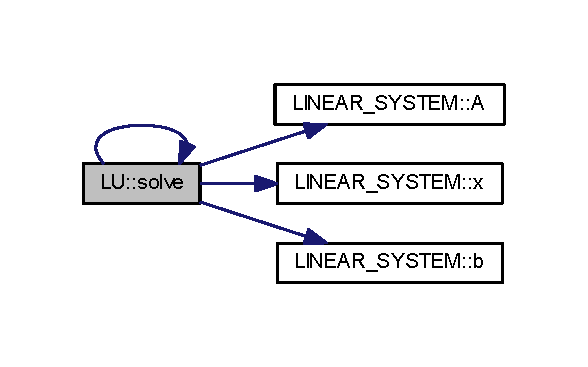
\includegraphics[width=282pt]{class_l_u_a624d7ff38645debae206313534516f49_cgraph}
\end{center}
\end{figure}
Here is the caller graph for this function\+:
\nopagebreak
\begin{figure}[H]
\begin{center}
\leavevmode
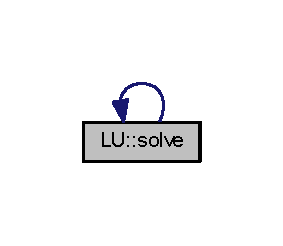
\includegraphics[width=136pt]{class_l_u_a624d7ff38645debae206313534516f49_icgraph}
\end{center}
\end{figure}


The documentation for this class was generated from the following file\+:\begin{DoxyCompactItemize}
\item 
\mbox{\hyperlink{lin__sys_8h}{lin\+\_\+sys.\+h}}\end{DoxyCompactItemize}

\hypertarget{class_module}{}\section{Module Class Reference}
\label{class_module}\index{Module@{Module}}


Akstrakte Klasse für allgemeine Bauteile.  




{\ttfamily \#include $<$module.\+h$>$}



Inheritance diagram for Module\+:\nopagebreak
\begin{figure}[H]
\begin{center}
\leavevmode
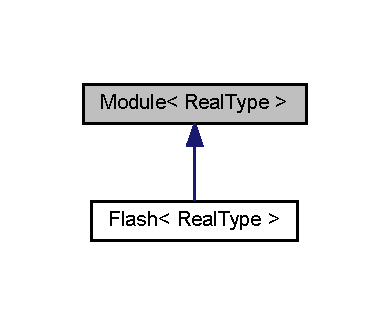
\includegraphics[width=128pt]{class_module__inherit__graph}
\end{center}
\end{figure}
\subsection*{Public Member Functions}
\begin{DoxyCompactItemize}
\item 
\mbox{\hyperlink{class_module_a5a240a8a9ab1813b17bcb810b24ceaea}{Module}} ()
\end{DoxyCompactItemize}


\subsection{Detailed Description}
Akstrakte Klasse für allgemeine Bauteile. 

Diese Klasse ist eine allgemeine Klasse, welche die In-\/ und Outputs definiert und die innere Operation abstrakt lässt. 

\subsection{Constructor \& Destructor Documentation}
\mbox{\Hypertarget{class_module_a5a240a8a9ab1813b17bcb810b24ceaea}\label{class_module_a5a240a8a9ab1813b17bcb810b24ceaea}} 
\index{Module@{Module}!Module@{Module}}
\index{Module@{Module}!Module@{Module}}
\subsubsection{\texorpdfstring{Module()}{Module()}}
{\footnotesize\ttfamily Module\+::\+Module (\begin{DoxyParamCaption}{ }\end{DoxyParamCaption})}



The documentation for this class was generated from the following files\+:\begin{DoxyCompactItemize}
\item 
\mbox{\hyperlink{module_8h}{module.\+h}}\item 
\mbox{\hyperlink{module_8cpp}{module.\+cpp}}\end{DoxyCompactItemize}

\hypertarget{class_n_e_w_t_o_n}{}\section{N\+E\+W\+T\+ON$<$ TS, NP, NS, TP $>$ Class Template Reference}
\label{class_n_e_w_t_o_n}\index{N\+E\+W\+T\+O\+N$<$ T\+S, N\+P, N\+S, T\+P $>$@{N\+E\+W\+T\+O\+N$<$ T\+S, N\+P, N\+S, T\+P $>$}}


{\ttfamily \#include $<$nonlin\+\_\+sys.\+h$>$}



Inheritance diagram for N\+E\+W\+T\+ON$<$ TS, NP, NS, TP $>$\+:\nopagebreak
\begin{figure}[H]
\begin{center}
\leavevmode
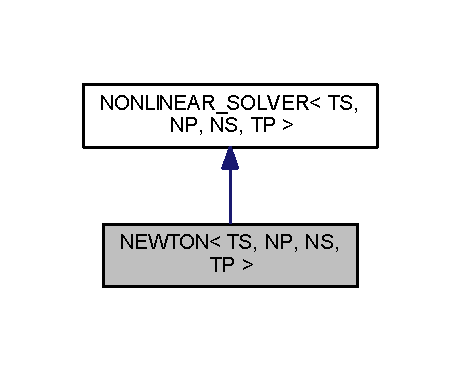
\includegraphics[width=221pt]{class_n_e_w_t_o_n__inherit__graph}
\end{center}
\end{figure}


Collaboration diagram for N\+E\+W\+T\+ON$<$ TS, NP, NS, TP $>$\+:\nopagebreak
\begin{figure}[H]
\begin{center}
\leavevmode
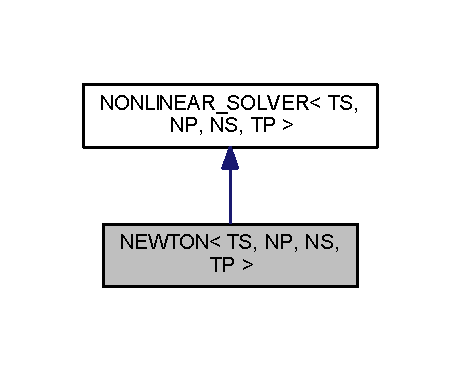
\includegraphics[width=221pt]{class_n_e_w_t_o_n__coll__graph}
\end{center}
\end{figure}
\subsection*{Public Member Functions}
\begin{DoxyCompactItemize}
\item 
\mbox{\hyperlink{class_n_e_w_t_o_n_a473d598fe7f30d8895a90a7daecb5f01}{N\+E\+W\+T\+ON}} (\mbox{\hyperlink{class_l_i_n_e_a_r___s_o_l_v_e_r}{L\+I\+N\+E\+A\+R\+\_\+\+S\+O\+L\+V\+ER}}$<$ TS, NS $>$ \&lsol)
\item 
double \& \mbox{\hyperlink{class_n_e_w_t_o_n_a222247d7695d9cce96f424a49d5ad2f6}{eps}} ()
\item 
void \mbox{\hyperlink{class_n_e_w_t_o_n_a1dd31b882567d3e0427eb53ce169f0ce}{solve}} (\mbox{\hyperlink{class_n_o_n_l_i_n_e_a_r___s_y_s_t_e_m}{N\+O\+N\+L\+I\+N\+E\+A\+R\+\_\+\+S\+Y\+S\+T\+EM}}$<$ TS, NP, NS, TP $>$ \&nlsys)
\end{DoxyCompactItemize}


\subsection{Constructor \& Destructor Documentation}
\mbox{\Hypertarget{class_n_e_w_t_o_n_a473d598fe7f30d8895a90a7daecb5f01}\label{class_n_e_w_t_o_n_a473d598fe7f30d8895a90a7daecb5f01}} 
\index{N\+E\+W\+T\+ON@{N\+E\+W\+T\+ON}!N\+E\+W\+T\+ON@{N\+E\+W\+T\+ON}}
\index{N\+E\+W\+T\+ON@{N\+E\+W\+T\+ON}!N\+E\+W\+T\+ON@{N\+E\+W\+T\+ON}}
\subsubsection{\texorpdfstring{N\+E\+W\+T\+O\+N()}{NEWTON()}}
{\footnotesize\ttfamily template$<$typename TS  = double, int NP = Dynamic, int NS = Dynamic, typename TP  = TS$>$ \\
\mbox{\hyperlink{class_n_e_w_t_o_n}{N\+E\+W\+T\+ON}}$<$ TS, NP, NS, TP $>$\+::\mbox{\hyperlink{class_n_e_w_t_o_n}{N\+E\+W\+T\+ON}} (\begin{DoxyParamCaption}\item[{\mbox{\hyperlink{class_l_i_n_e_a_r___s_o_l_v_e_r}{L\+I\+N\+E\+A\+R\+\_\+\+S\+O\+L\+V\+ER}}$<$ TS, NS $>$ \&}]{lsol }\end{DoxyParamCaption})\hspace{0.3cm}{\ttfamily [inline]}}



\subsection{Member Function Documentation}
\mbox{\Hypertarget{class_n_e_w_t_o_n_a222247d7695d9cce96f424a49d5ad2f6}\label{class_n_e_w_t_o_n_a222247d7695d9cce96f424a49d5ad2f6}} 
\index{N\+E\+W\+T\+ON@{N\+E\+W\+T\+ON}!eps@{eps}}
\index{eps@{eps}!N\+E\+W\+T\+ON@{N\+E\+W\+T\+ON}}
\subsubsection{\texorpdfstring{eps()}{eps()}}
{\footnotesize\ttfamily template$<$typename TS  = double, int NP = Dynamic, int NS = Dynamic, typename TP  = TS$>$ \\
double\& \mbox{\hyperlink{class_n_e_w_t_o_n}{N\+E\+W\+T\+ON}}$<$ TS, NP, NS, TP $>$\+::eps (\begin{DoxyParamCaption}{ }\end{DoxyParamCaption})\hspace{0.3cm}{\ttfamily [inline]}}

\mbox{\Hypertarget{class_n_e_w_t_o_n_a1dd31b882567d3e0427eb53ce169f0ce}\label{class_n_e_w_t_o_n_a1dd31b882567d3e0427eb53ce169f0ce}} 
\index{N\+E\+W\+T\+ON@{N\+E\+W\+T\+ON}!solve@{solve}}
\index{solve@{solve}!N\+E\+W\+T\+ON@{N\+E\+W\+T\+ON}}
\subsubsection{\texorpdfstring{solve()}{solve()}}
{\footnotesize\ttfamily template$<$typename TS  = double, int NP = Dynamic, int NS = Dynamic, typename TP  = TS$>$ \\
void \mbox{\hyperlink{class_n_e_w_t_o_n}{N\+E\+W\+T\+ON}}$<$ TS, NP, NS, TP $>$\+::solve (\begin{DoxyParamCaption}\item[{\mbox{\hyperlink{class_n_o_n_l_i_n_e_a_r___s_y_s_t_e_m}{N\+O\+N\+L\+I\+N\+E\+A\+R\+\_\+\+S\+Y\+S\+T\+EM}}$<$ TS, NP, NS, TP $>$ \&}]{nlsys }\end{DoxyParamCaption})\hspace{0.3cm}{\ttfamily [inline]}, {\ttfamily [virtual]}}



Implements \mbox{\hyperlink{class_n_o_n_l_i_n_e_a_r___s_o_l_v_e_r_aae333fb75e2d5d8baa0e37991bfac7c4}{N\+O\+N\+L\+I\+N\+E\+A\+R\+\_\+\+S\+O\+L\+V\+E\+R$<$ T\+S, N\+P, N\+S, T\+P $>$}}.

Here is the call graph for this function\+:
\nopagebreak
\begin{figure}[H]
\begin{center}
\leavevmode
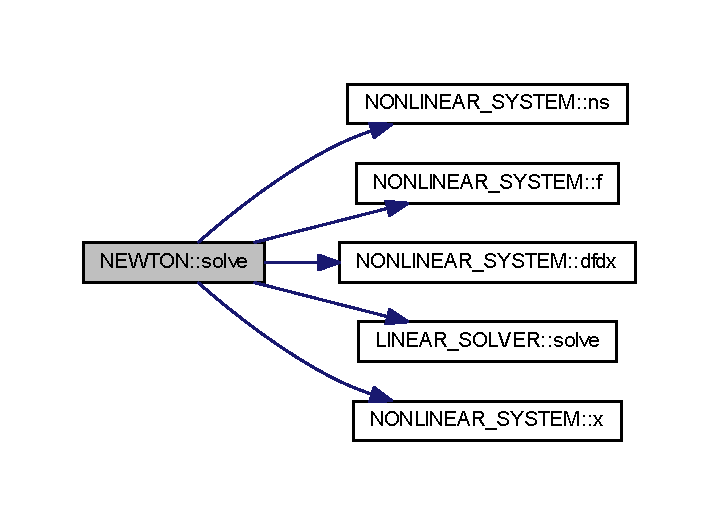
\includegraphics[width=345pt]{class_n_e_w_t_o_n_a1dd31b882567d3e0427eb53ce169f0ce_cgraph}
\end{center}
\end{figure}


The documentation for this class was generated from the following file\+:\begin{DoxyCompactItemize}
\item 
\mbox{\hyperlink{nonlin__sys_8h}{nonlin\+\_\+sys.\+h}}\end{DoxyCompactItemize}

\hypertarget{class_n_o_n_l_i_n_e_a_r___s_o_l_v_e_r}{}\section{N\+O\+N\+L\+I\+N\+E\+A\+R\+\_\+\+S\+O\+L\+V\+ER$<$ TS, NP, NS, TP $>$ Class Template Reference}
\label{class_n_o_n_l_i_n_e_a_r___s_o_l_v_e_r}\index{N\+O\+N\+L\+I\+N\+E\+A\+R\+\_\+\+S\+O\+L\+V\+E\+R$<$ T\+S, N\+P, N\+S, T\+P $>$@{N\+O\+N\+L\+I\+N\+E\+A\+R\+\_\+\+S\+O\+L\+V\+E\+R$<$ T\+S, N\+P, N\+S, T\+P $>$}}


{\ttfamily \#include $<$nonlin\+\_\+sys.\+h$>$}



Inheritance diagram for N\+O\+N\+L\+I\+N\+E\+A\+R\+\_\+\+S\+O\+L\+V\+ER$<$ TS, NP, NS, TP $>$\+:\nopagebreak
\begin{figure}[H]
\begin{center}
\leavevmode
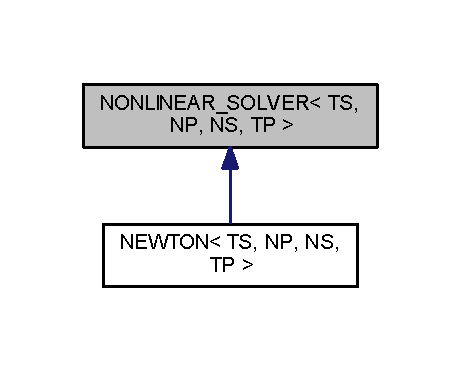
\includegraphics[width=221pt]{class_n_o_n_l_i_n_e_a_r___s_o_l_v_e_r__inherit__graph}
\end{center}
\end{figure}
\subsection*{Public Member Functions}
\begin{DoxyCompactItemize}
\item 
virtual void \mbox{\hyperlink{class_n_o_n_l_i_n_e_a_r___s_o_l_v_e_r_aae333fb75e2d5d8baa0e37991bfac7c4}{solve}} (\mbox{\hyperlink{class_n_o_n_l_i_n_e_a_r___s_y_s_t_e_m}{N\+O\+N\+L\+I\+N\+E\+A\+R\+\_\+\+S\+Y\+S\+T\+EM}}$<$ TS, NP, NS, TP $>$ \&)=0
\end{DoxyCompactItemize}


\subsection{Member Function Documentation}
\mbox{\Hypertarget{class_n_o_n_l_i_n_e_a_r___s_o_l_v_e_r_aae333fb75e2d5d8baa0e37991bfac7c4}\label{class_n_o_n_l_i_n_e_a_r___s_o_l_v_e_r_aae333fb75e2d5d8baa0e37991bfac7c4}} 
\index{N\+O\+N\+L\+I\+N\+E\+A\+R\+\_\+\+S\+O\+L\+V\+ER@{N\+O\+N\+L\+I\+N\+E\+A\+R\+\_\+\+S\+O\+L\+V\+ER}!solve@{solve}}
\index{solve@{solve}!N\+O\+N\+L\+I\+N\+E\+A\+R\+\_\+\+S\+O\+L\+V\+ER@{N\+O\+N\+L\+I\+N\+E\+A\+R\+\_\+\+S\+O\+L\+V\+ER}}
\subsubsection{\texorpdfstring{solve()}{solve()}}
{\footnotesize\ttfamily template$<$typename TS  = double, int NP = Dynamic, int NS = Dynamic, typename TP  = TS$>$ \\
virtual void \mbox{\hyperlink{class_n_o_n_l_i_n_e_a_r___s_o_l_v_e_r}{N\+O\+N\+L\+I\+N\+E\+A\+R\+\_\+\+S\+O\+L\+V\+ER}}$<$ TS, NP, NS, TP $>$\+::solve (\begin{DoxyParamCaption}\item[{\mbox{\hyperlink{class_n_o_n_l_i_n_e_a_r___s_y_s_t_e_m}{N\+O\+N\+L\+I\+N\+E\+A\+R\+\_\+\+S\+Y\+S\+T\+EM}}$<$ TS, NP, NS, TP $>$ \&}]{ }\end{DoxyParamCaption})\hspace{0.3cm}{\ttfamily [pure virtual]}}



Implemented in \mbox{\hyperlink{class_n_e_w_t_o_n_a1dd31b882567d3e0427eb53ce169f0ce}{N\+E\+W\+T\+O\+N$<$ T\+S, N\+P, N\+S, T\+P $>$}}.



The documentation for this class was generated from the following file\+:\begin{DoxyCompactItemize}
\item 
\mbox{\hyperlink{nonlin__sys_8h}{nonlin\+\_\+sys.\+h}}\end{DoxyCompactItemize}

\hypertarget{class_n_o_n_l_i_n_e_a_r___s_y_s_t_e_m}{}\section{N\+O\+N\+L\+I\+N\+E\+A\+R\+\_\+\+S\+Y\+S\+T\+EM$<$ TS, NP, NS, TP $>$ Class Template Reference}
\label{class_n_o_n_l_i_n_e_a_r___s_y_s_t_e_m}\index{N\+O\+N\+L\+I\+N\+E\+A\+R\+\_\+\+S\+Y\+S\+T\+E\+M$<$ T\+S, N\+P, N\+S, T\+P $>$@{N\+O\+N\+L\+I\+N\+E\+A\+R\+\_\+\+S\+Y\+S\+T\+E\+M$<$ T\+S, N\+P, N\+S, T\+P $>$}}


Nichtlineare Systeme Basierend auf \mbox{\hyperlink{nonlin__sys_8h}{nonlin\+\_\+sys.\+h}} von Uwe Naumann.  




{\ttfamily \#include $<$nonlin\+\_\+sys.\+h$>$}



Inheritance diagram for N\+O\+N\+L\+I\+N\+E\+A\+R\+\_\+\+S\+Y\+S\+T\+EM$<$ TS, NP, NS, TP $>$\+:\nopagebreak
\begin{figure}[H]
\begin{center}
\leavevmode
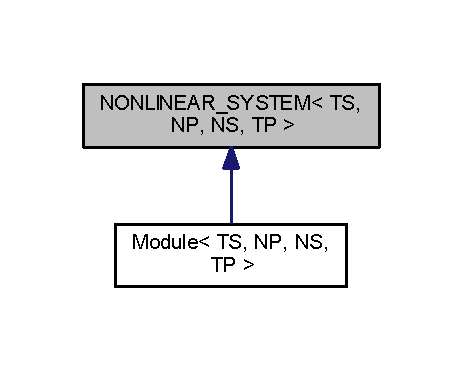
\includegraphics[width=326pt]{class_n_o_n_l_i_n_e_a_r___s_y_s_t_e_m__inherit__graph}
\end{center}
\end{figure}
\subsection*{Public Member Functions}
\begin{DoxyCompactItemize}
\item 
\mbox{\hyperlink{class_n_o_n_l_i_n_e_a_r___s_y_s_t_e_m_aa6073542adb090bf99729df5b03ca707}{N\+O\+N\+L\+I\+N\+E\+A\+R\+\_\+\+S\+Y\+S\+T\+EM}} (int \mbox{\hyperlink{class_n_o_n_l_i_n_e_a_r___s_y_s_t_e_m_ab5876470030832088d8ee1ed609d5311}{np}}, int \mbox{\hyperlink{class_n_o_n_l_i_n_e_a_r___s_y_s_t_e_m_abf4102c649f8316e44033a76f9d6183f}{ns}})
\item 
int \mbox{\hyperlink{class_n_o_n_l_i_n_e_a_r___s_y_s_t_e_m_abf4102c649f8316e44033a76f9d6183f}{ns}} ()
\item 
int \mbox{\hyperlink{class_n_o_n_l_i_n_e_a_r___s_y_s_t_e_m_ab5876470030832088d8ee1ed609d5311}{np}} ()
\item 
V\+TS \& \mbox{\hyperlink{class_n_o_n_l_i_n_e_a_r___s_y_s_t_e_m_a74d8eaa53624eae38a6f2e6b5bdd4381}{x}} ()
\item 
TS \& \mbox{\hyperlink{class_n_o_n_l_i_n_e_a_r___s_y_s_t_e_m_aabd6041ce7d6aaad8ce55e03c2efde1e}{x}} (int i)
\item 
V\+TP \& \mbox{\hyperlink{class_n_o_n_l_i_n_e_a_r___s_y_s_t_e_m_a1536a98a6cb3fec681bdd3312ae43714}{p}} ()
\item 
TP \& \mbox{\hyperlink{class_n_o_n_l_i_n_e_a_r___s_y_s_t_e_m_a75739c8370b0aa04f8f03e88ac19d09b}{p}} (int i)
\item 
virtual V\+TS \mbox{\hyperlink{class_n_o_n_l_i_n_e_a_r___s_y_s_t_e_m_a65827d7df297f26cd3f14f472a212077}{f}} ()=0
\item 
virtual M\+TS \mbox{\hyperlink{class_n_o_n_l_i_n_e_a_r___s_y_s_t_e_m_a531f56bcbc77f2219164af40aa16fad2}{dfdx}} ()=0
\end{DoxyCompactItemize}
\subsection*{Protected Attributes}
\begin{DoxyCompactItemize}
\item 
V\+TS \mbox{\hyperlink{class_n_o_n_l_i_n_e_a_r___s_y_s_t_e_m_a06e2289a0e10aa47527d5fd348faf4f9}{\+\_\+x}}
\item 
V\+TP \mbox{\hyperlink{class_n_o_n_l_i_n_e_a_r___s_y_s_t_e_m_aee48110f36d056d217437af5e7cc5447}{\+\_\+p}}
\end{DoxyCompactItemize}


\subsection{Detailed Description}
\subsubsection*{template$<$typename TS = double, int NP = Dynamic, int NS = Dynamic, typename TP = TS$>$\newline
class N\+O\+N\+L\+I\+N\+E\+A\+R\+\_\+\+S\+Y\+S\+T\+E\+M$<$ T\+S, N\+P, N\+S, T\+P $>$}

Nichtlineare Systeme Basierend auf \mbox{\hyperlink{nonlin__sys_8h}{nonlin\+\_\+sys.\+h}} von Uwe Naumann. 

\subsection{Constructor \& Destructor Documentation}
\mbox{\Hypertarget{class_n_o_n_l_i_n_e_a_r___s_y_s_t_e_m_aa6073542adb090bf99729df5b03ca707}\label{class_n_o_n_l_i_n_e_a_r___s_y_s_t_e_m_aa6073542adb090bf99729df5b03ca707}} 
\index{N\+O\+N\+L\+I\+N\+E\+A\+R\+\_\+\+S\+Y\+S\+T\+EM@{N\+O\+N\+L\+I\+N\+E\+A\+R\+\_\+\+S\+Y\+S\+T\+EM}!N\+O\+N\+L\+I\+N\+E\+A\+R\+\_\+\+S\+Y\+S\+T\+EM@{N\+O\+N\+L\+I\+N\+E\+A\+R\+\_\+\+S\+Y\+S\+T\+EM}}
\index{N\+O\+N\+L\+I\+N\+E\+A\+R\+\_\+\+S\+Y\+S\+T\+EM@{N\+O\+N\+L\+I\+N\+E\+A\+R\+\_\+\+S\+Y\+S\+T\+EM}!N\+O\+N\+L\+I\+N\+E\+A\+R\+\_\+\+S\+Y\+S\+T\+EM@{N\+O\+N\+L\+I\+N\+E\+A\+R\+\_\+\+S\+Y\+S\+T\+EM}}
\subsubsection{\texorpdfstring{N\+O\+N\+L\+I\+N\+E\+A\+R\+\_\+\+S\+Y\+S\+T\+E\+M()}{NONLINEAR\_SYSTEM()}}
{\footnotesize\ttfamily template$<$typename TS = double, int NP = Dynamic, int NS = Dynamic, typename TP = TS$>$ \\
\mbox{\hyperlink{class_n_o_n_l_i_n_e_a_r___s_y_s_t_e_m}{N\+O\+N\+L\+I\+N\+E\+A\+R\+\_\+\+S\+Y\+S\+T\+EM}}$<$ TS, NP, NS, TP $>$\+::\mbox{\hyperlink{class_n_o_n_l_i_n_e_a_r___s_y_s_t_e_m}{N\+O\+N\+L\+I\+N\+E\+A\+R\+\_\+\+S\+Y\+S\+T\+EM}} (\begin{DoxyParamCaption}\item[{int}]{np,  }\item[{int}]{ns }\end{DoxyParamCaption})\hspace{0.3cm}{\ttfamily [inline]}}



\subsection{Member Function Documentation}
\mbox{\Hypertarget{class_n_o_n_l_i_n_e_a_r___s_y_s_t_e_m_a531f56bcbc77f2219164af40aa16fad2}\label{class_n_o_n_l_i_n_e_a_r___s_y_s_t_e_m_a531f56bcbc77f2219164af40aa16fad2}} 
\index{N\+O\+N\+L\+I\+N\+E\+A\+R\+\_\+\+S\+Y\+S\+T\+EM@{N\+O\+N\+L\+I\+N\+E\+A\+R\+\_\+\+S\+Y\+S\+T\+EM}!dfdx@{dfdx}}
\index{dfdx@{dfdx}!N\+O\+N\+L\+I\+N\+E\+A\+R\+\_\+\+S\+Y\+S\+T\+EM@{N\+O\+N\+L\+I\+N\+E\+A\+R\+\_\+\+S\+Y\+S\+T\+EM}}
\subsubsection{\texorpdfstring{dfdx()}{dfdx()}}
{\footnotesize\ttfamily template$<$typename TS = double, int NP = Dynamic, int NS = Dynamic, typename TP = TS$>$ \\
virtual M\+TS \mbox{\hyperlink{class_n_o_n_l_i_n_e_a_r___s_y_s_t_e_m}{N\+O\+N\+L\+I\+N\+E\+A\+R\+\_\+\+S\+Y\+S\+T\+EM}}$<$ TS, NP, NS, TP $>$\+::dfdx (\begin{DoxyParamCaption}{ }\end{DoxyParamCaption})\hspace{0.3cm}{\ttfamily [pure virtual]}}



Implemented in \mbox{\hyperlink{class_flash_a83e35b3ab13b3705f0fe06c40b800a8b}{Flash$<$ T\+S, N\+P, N\+S, T\+P $>$}}, and \mbox{\hyperlink{classcascade_ac72705f0ad01cc88d43c002d63acce13}{cascade$<$ T\+S, N\+P, N\+S, T\+P $>$}}.

Here is the caller graph for this function\+:\nopagebreak
\begin{figure}[H]
\begin{center}
\leavevmode
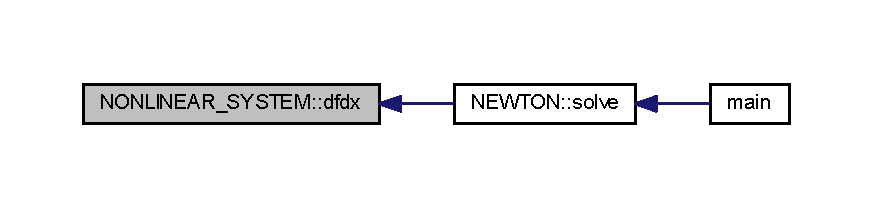
\includegraphics[width=350pt]{class_n_o_n_l_i_n_e_a_r___s_y_s_t_e_m_a531f56bcbc77f2219164af40aa16fad2_icgraph}
\end{center}
\end{figure}
\mbox{\Hypertarget{class_n_o_n_l_i_n_e_a_r___s_y_s_t_e_m_a65827d7df297f26cd3f14f472a212077}\label{class_n_o_n_l_i_n_e_a_r___s_y_s_t_e_m_a65827d7df297f26cd3f14f472a212077}} 
\index{N\+O\+N\+L\+I\+N\+E\+A\+R\+\_\+\+S\+Y\+S\+T\+EM@{N\+O\+N\+L\+I\+N\+E\+A\+R\+\_\+\+S\+Y\+S\+T\+EM}!f@{f}}
\index{f@{f}!N\+O\+N\+L\+I\+N\+E\+A\+R\+\_\+\+S\+Y\+S\+T\+EM@{N\+O\+N\+L\+I\+N\+E\+A\+R\+\_\+\+S\+Y\+S\+T\+EM}}
\subsubsection{\texorpdfstring{f()}{f()}}
{\footnotesize\ttfamily template$<$typename TS = double, int NP = Dynamic, int NS = Dynamic, typename TP = TS$>$ \\
virtual V\+TS \mbox{\hyperlink{class_n_o_n_l_i_n_e_a_r___s_y_s_t_e_m}{N\+O\+N\+L\+I\+N\+E\+A\+R\+\_\+\+S\+Y\+S\+T\+EM}}$<$ TS, NP, NS, TP $>$\+::f (\begin{DoxyParamCaption}{ }\end{DoxyParamCaption})\hspace{0.3cm}{\ttfamily [pure virtual]}}



Implemented in \mbox{\hyperlink{class_flash_ad29e755877ca96aa5b9f34a10d6cd8b2}{Flash$<$ T\+S, N\+P, N\+S, T\+P $>$}}, and \mbox{\hyperlink{classcascade_a9c5bb14ea8b17d1f79c097c6704f1919}{cascade$<$ T\+S, N\+P, N\+S, T\+P $>$}}.

Here is the caller graph for this function\+:\nopagebreak
\begin{figure}[H]
\begin{center}
\leavevmode
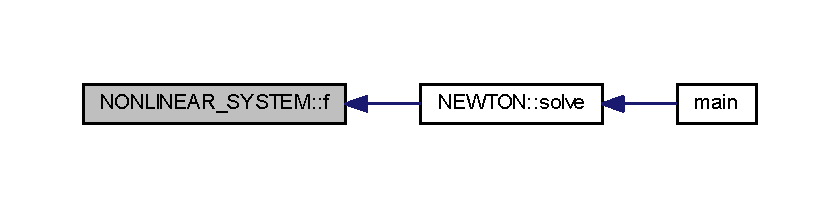
\includegraphics[width=350pt]{class_n_o_n_l_i_n_e_a_r___s_y_s_t_e_m_a65827d7df297f26cd3f14f472a212077_icgraph}
\end{center}
\end{figure}
\mbox{\Hypertarget{class_n_o_n_l_i_n_e_a_r___s_y_s_t_e_m_ab5876470030832088d8ee1ed609d5311}\label{class_n_o_n_l_i_n_e_a_r___s_y_s_t_e_m_ab5876470030832088d8ee1ed609d5311}} 
\index{N\+O\+N\+L\+I\+N\+E\+A\+R\+\_\+\+S\+Y\+S\+T\+EM@{N\+O\+N\+L\+I\+N\+E\+A\+R\+\_\+\+S\+Y\+S\+T\+EM}!np@{np}}
\index{np@{np}!N\+O\+N\+L\+I\+N\+E\+A\+R\+\_\+\+S\+Y\+S\+T\+EM@{N\+O\+N\+L\+I\+N\+E\+A\+R\+\_\+\+S\+Y\+S\+T\+EM}}
\subsubsection{\texorpdfstring{np()}{np()}}
{\footnotesize\ttfamily template$<$typename TS = double, int NP = Dynamic, int NS = Dynamic, typename TP = TS$>$ \\
int \mbox{\hyperlink{class_n_o_n_l_i_n_e_a_r___s_y_s_t_e_m}{N\+O\+N\+L\+I\+N\+E\+A\+R\+\_\+\+S\+Y\+S\+T\+EM}}$<$ TS, NP, NS, TP $>$\+::np (\begin{DoxyParamCaption}{ }\end{DoxyParamCaption})\hspace{0.3cm}{\ttfamily [inline]}}

\mbox{\Hypertarget{class_n_o_n_l_i_n_e_a_r___s_y_s_t_e_m_abf4102c649f8316e44033a76f9d6183f}\label{class_n_o_n_l_i_n_e_a_r___s_y_s_t_e_m_abf4102c649f8316e44033a76f9d6183f}} 
\index{N\+O\+N\+L\+I\+N\+E\+A\+R\+\_\+\+S\+Y\+S\+T\+EM@{N\+O\+N\+L\+I\+N\+E\+A\+R\+\_\+\+S\+Y\+S\+T\+EM}!ns@{ns}}
\index{ns@{ns}!N\+O\+N\+L\+I\+N\+E\+A\+R\+\_\+\+S\+Y\+S\+T\+EM@{N\+O\+N\+L\+I\+N\+E\+A\+R\+\_\+\+S\+Y\+S\+T\+EM}}
\subsubsection{\texorpdfstring{ns()}{ns()}}
{\footnotesize\ttfamily template$<$typename TS = double, int NP = Dynamic, int NS = Dynamic, typename TP = TS$>$ \\
int \mbox{\hyperlink{class_n_o_n_l_i_n_e_a_r___s_y_s_t_e_m}{N\+O\+N\+L\+I\+N\+E\+A\+R\+\_\+\+S\+Y\+S\+T\+EM}}$<$ TS, NP, NS, TP $>$\+::ns (\begin{DoxyParamCaption}{ }\end{DoxyParamCaption})\hspace{0.3cm}{\ttfamily [inline]}}

Here is the caller graph for this function\+:\nopagebreak
\begin{figure}[H]
\begin{center}
\leavevmode
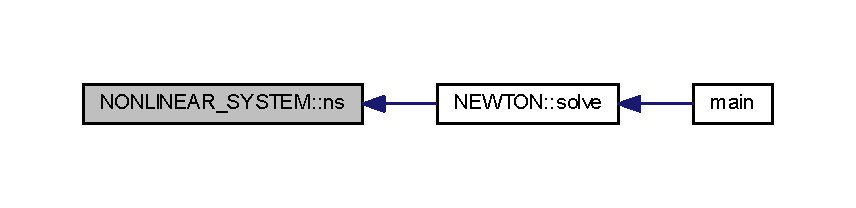
\includegraphics[width=350pt]{class_n_o_n_l_i_n_e_a_r___s_y_s_t_e_m_abf4102c649f8316e44033a76f9d6183f_icgraph}
\end{center}
\end{figure}
\mbox{\Hypertarget{class_n_o_n_l_i_n_e_a_r___s_y_s_t_e_m_a1536a98a6cb3fec681bdd3312ae43714}\label{class_n_o_n_l_i_n_e_a_r___s_y_s_t_e_m_a1536a98a6cb3fec681bdd3312ae43714}} 
\index{N\+O\+N\+L\+I\+N\+E\+A\+R\+\_\+\+S\+Y\+S\+T\+EM@{N\+O\+N\+L\+I\+N\+E\+A\+R\+\_\+\+S\+Y\+S\+T\+EM}!p@{p}}
\index{p@{p}!N\+O\+N\+L\+I\+N\+E\+A\+R\+\_\+\+S\+Y\+S\+T\+EM@{N\+O\+N\+L\+I\+N\+E\+A\+R\+\_\+\+S\+Y\+S\+T\+EM}}
\subsubsection{\texorpdfstring{p()}{p()}\hspace{0.1cm}{\footnotesize\ttfamily [1/2]}}
{\footnotesize\ttfamily template$<$typename TS = double, int NP = Dynamic, int NS = Dynamic, typename TP = TS$>$ \\
V\+TP\& \mbox{\hyperlink{class_n_o_n_l_i_n_e_a_r___s_y_s_t_e_m}{N\+O\+N\+L\+I\+N\+E\+A\+R\+\_\+\+S\+Y\+S\+T\+EM}}$<$ TS, NP, NS, TP $>$\+::p (\begin{DoxyParamCaption}{ }\end{DoxyParamCaption})\hspace{0.3cm}{\ttfamily [inline]}}

\mbox{\Hypertarget{class_n_o_n_l_i_n_e_a_r___s_y_s_t_e_m_a75739c8370b0aa04f8f03e88ac19d09b}\label{class_n_o_n_l_i_n_e_a_r___s_y_s_t_e_m_a75739c8370b0aa04f8f03e88ac19d09b}} 
\index{N\+O\+N\+L\+I\+N\+E\+A\+R\+\_\+\+S\+Y\+S\+T\+EM@{N\+O\+N\+L\+I\+N\+E\+A\+R\+\_\+\+S\+Y\+S\+T\+EM}!p@{p}}
\index{p@{p}!N\+O\+N\+L\+I\+N\+E\+A\+R\+\_\+\+S\+Y\+S\+T\+EM@{N\+O\+N\+L\+I\+N\+E\+A\+R\+\_\+\+S\+Y\+S\+T\+EM}}
\subsubsection{\texorpdfstring{p()}{p()}\hspace{0.1cm}{\footnotesize\ttfamily [2/2]}}
{\footnotesize\ttfamily template$<$typename TS = double, int NP = Dynamic, int NS = Dynamic, typename TP = TS$>$ \\
TP\& \mbox{\hyperlink{class_n_o_n_l_i_n_e_a_r___s_y_s_t_e_m}{N\+O\+N\+L\+I\+N\+E\+A\+R\+\_\+\+S\+Y\+S\+T\+EM}}$<$ TS, NP, NS, TP $>$\+::p (\begin{DoxyParamCaption}\item[{int}]{i }\end{DoxyParamCaption})\hspace{0.3cm}{\ttfamily [inline]}}

\mbox{\Hypertarget{class_n_o_n_l_i_n_e_a_r___s_y_s_t_e_m_a74d8eaa53624eae38a6f2e6b5bdd4381}\label{class_n_o_n_l_i_n_e_a_r___s_y_s_t_e_m_a74d8eaa53624eae38a6f2e6b5bdd4381}} 
\index{N\+O\+N\+L\+I\+N\+E\+A\+R\+\_\+\+S\+Y\+S\+T\+EM@{N\+O\+N\+L\+I\+N\+E\+A\+R\+\_\+\+S\+Y\+S\+T\+EM}!x@{x}}
\index{x@{x}!N\+O\+N\+L\+I\+N\+E\+A\+R\+\_\+\+S\+Y\+S\+T\+EM@{N\+O\+N\+L\+I\+N\+E\+A\+R\+\_\+\+S\+Y\+S\+T\+EM}}
\subsubsection{\texorpdfstring{x()}{x()}\hspace{0.1cm}{\footnotesize\ttfamily [1/2]}}
{\footnotesize\ttfamily template$<$typename TS = double, int NP = Dynamic, int NS = Dynamic, typename TP = TS$>$ \\
V\+TS\& \mbox{\hyperlink{class_n_o_n_l_i_n_e_a_r___s_y_s_t_e_m}{N\+O\+N\+L\+I\+N\+E\+A\+R\+\_\+\+S\+Y\+S\+T\+EM}}$<$ TS, NP, NS, TP $>$\+::x (\begin{DoxyParamCaption}{ }\end{DoxyParamCaption})\hspace{0.3cm}{\ttfamily [inline]}}

Here is the caller graph for this function\+:\nopagebreak
\begin{figure}[H]
\begin{center}
\leavevmode
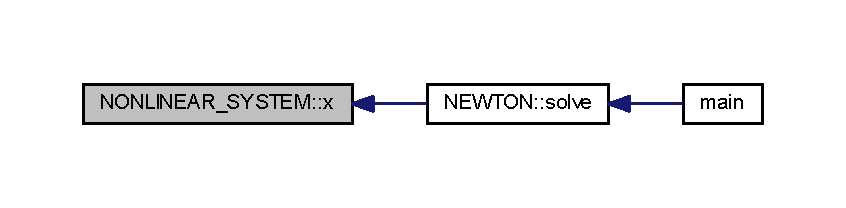
\includegraphics[width=350pt]{class_n_o_n_l_i_n_e_a_r___s_y_s_t_e_m_a74d8eaa53624eae38a6f2e6b5bdd4381_icgraph}
\end{center}
\end{figure}
\mbox{\Hypertarget{class_n_o_n_l_i_n_e_a_r___s_y_s_t_e_m_aabd6041ce7d6aaad8ce55e03c2efde1e}\label{class_n_o_n_l_i_n_e_a_r___s_y_s_t_e_m_aabd6041ce7d6aaad8ce55e03c2efde1e}} 
\index{N\+O\+N\+L\+I\+N\+E\+A\+R\+\_\+\+S\+Y\+S\+T\+EM@{N\+O\+N\+L\+I\+N\+E\+A\+R\+\_\+\+S\+Y\+S\+T\+EM}!x@{x}}
\index{x@{x}!N\+O\+N\+L\+I\+N\+E\+A\+R\+\_\+\+S\+Y\+S\+T\+EM@{N\+O\+N\+L\+I\+N\+E\+A\+R\+\_\+\+S\+Y\+S\+T\+EM}}
\subsubsection{\texorpdfstring{x()}{x()}\hspace{0.1cm}{\footnotesize\ttfamily [2/2]}}
{\footnotesize\ttfamily template$<$typename TS = double, int NP = Dynamic, int NS = Dynamic, typename TP = TS$>$ \\
TS\& \mbox{\hyperlink{class_n_o_n_l_i_n_e_a_r___s_y_s_t_e_m}{N\+O\+N\+L\+I\+N\+E\+A\+R\+\_\+\+S\+Y\+S\+T\+EM}}$<$ TS, NP, NS, TP $>$\+::x (\begin{DoxyParamCaption}\item[{int}]{i }\end{DoxyParamCaption})\hspace{0.3cm}{\ttfamily [inline]}}



\subsection{Member Data Documentation}
\mbox{\Hypertarget{class_n_o_n_l_i_n_e_a_r___s_y_s_t_e_m_aee48110f36d056d217437af5e7cc5447}\label{class_n_o_n_l_i_n_e_a_r___s_y_s_t_e_m_aee48110f36d056d217437af5e7cc5447}} 
\index{N\+O\+N\+L\+I\+N\+E\+A\+R\+\_\+\+S\+Y\+S\+T\+EM@{N\+O\+N\+L\+I\+N\+E\+A\+R\+\_\+\+S\+Y\+S\+T\+EM}!\+\_\+p@{\+\_\+p}}
\index{\+\_\+p@{\+\_\+p}!N\+O\+N\+L\+I\+N\+E\+A\+R\+\_\+\+S\+Y\+S\+T\+EM@{N\+O\+N\+L\+I\+N\+E\+A\+R\+\_\+\+S\+Y\+S\+T\+EM}}
\subsubsection{\texorpdfstring{\+\_\+p}{\_p}}
{\footnotesize\ttfamily template$<$typename TS = double, int NP = Dynamic, int NS = Dynamic, typename TP = TS$>$ \\
V\+TP \mbox{\hyperlink{class_n_o_n_l_i_n_e_a_r___s_y_s_t_e_m}{N\+O\+N\+L\+I\+N\+E\+A\+R\+\_\+\+S\+Y\+S\+T\+EM}}$<$ TS, NP, NS, TP $>$\+::\+\_\+p\hspace{0.3cm}{\ttfamily [protected]}}

\mbox{\Hypertarget{class_n_o_n_l_i_n_e_a_r___s_y_s_t_e_m_a06e2289a0e10aa47527d5fd348faf4f9}\label{class_n_o_n_l_i_n_e_a_r___s_y_s_t_e_m_a06e2289a0e10aa47527d5fd348faf4f9}} 
\index{N\+O\+N\+L\+I\+N\+E\+A\+R\+\_\+\+S\+Y\+S\+T\+EM@{N\+O\+N\+L\+I\+N\+E\+A\+R\+\_\+\+S\+Y\+S\+T\+EM}!\+\_\+x@{\+\_\+x}}
\index{\+\_\+x@{\+\_\+x}!N\+O\+N\+L\+I\+N\+E\+A\+R\+\_\+\+S\+Y\+S\+T\+EM@{N\+O\+N\+L\+I\+N\+E\+A\+R\+\_\+\+S\+Y\+S\+T\+EM}}
\subsubsection{\texorpdfstring{\+\_\+x}{\_x}}
{\footnotesize\ttfamily template$<$typename TS = double, int NP = Dynamic, int NS = Dynamic, typename TP = TS$>$ \\
V\+TS \mbox{\hyperlink{class_n_o_n_l_i_n_e_a_r___s_y_s_t_e_m}{N\+O\+N\+L\+I\+N\+E\+A\+R\+\_\+\+S\+Y\+S\+T\+EM}}$<$ TS, NP, NS, TP $>$\+::\+\_\+x\hspace{0.3cm}{\ttfamily [protected]}}



The documentation for this class was generated from the following file\+:\begin{DoxyCompactItemize}
\item 
\mbox{\hyperlink{nonlin__sys_8h}{nonlin\+\_\+sys.\+h}}\end{DoxyCompactItemize}

\hypertarget{class_q_r}{}\section{QR$<$ TA, N, Tb, Tx $>$ Class Template Reference}
\label{class_q_r}\index{Q\+R$<$ T\+A, N, Tb, Tx $>$@{Q\+R$<$ T\+A, N, Tb, Tx $>$}}


{\ttfamily \#include $<$lin\+\_\+sys.\+h$>$}



Inheritance diagram for QR$<$ TA, N, Tb, Tx $>$\+:\nopagebreak
\begin{figure}[H]
\begin{center}
\leavevmode
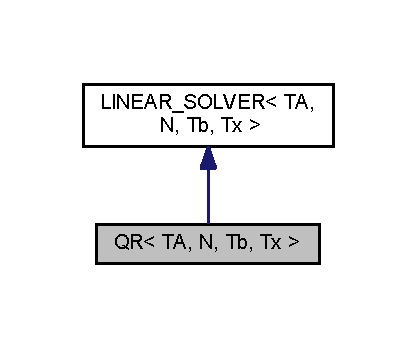
\includegraphics[width=200pt]{class_q_r__inherit__graph}
\end{center}
\end{figure}


Collaboration diagram for QR$<$ TA, N, Tb, Tx $>$\+:\nopagebreak
\begin{figure}[H]
\begin{center}
\leavevmode
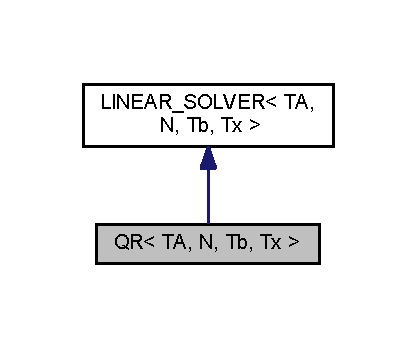
\includegraphics[width=200pt]{class_q_r__coll__graph}
\end{center}
\end{figure}
\subsection*{Public Member Functions}
\begin{DoxyCompactItemize}
\item 
void \mbox{\hyperlink{class_q_r_ab8f49cec36214bdcd9fca78e89c3737e}{solve}} (\mbox{\hyperlink{class_l_i_n_e_a_r___s_y_s_t_e_m}{L\+I\+N\+E\+A\+R\+\_\+\+S\+Y\+S\+T\+EM}}$<$ TA, N, Tb, Tx $>$ \&s)
\end{DoxyCompactItemize}


\subsection{Member Function Documentation}
\mbox{\Hypertarget{class_q_r_ab8f49cec36214bdcd9fca78e89c3737e}\label{class_q_r_ab8f49cec36214bdcd9fca78e89c3737e}} 
\index{QR@{QR}!solve@{solve}}
\index{solve@{solve}!QR@{QR}}
\subsubsection{\texorpdfstring{solve()}{solve()}}
{\footnotesize\ttfamily template$<$typename TA  = double, int N = Dynamic, typename Tb  = TA, typename Tx  = Tb$>$ \\
void \mbox{\hyperlink{class_q_r}{QR}}$<$ TA, N, Tb, Tx $>$\+::solve (\begin{DoxyParamCaption}\item[{\mbox{\hyperlink{class_l_i_n_e_a_r___s_y_s_t_e_m}{L\+I\+N\+E\+A\+R\+\_\+\+S\+Y\+S\+T\+EM}}$<$ TA, N, Tb, Tx $>$ \&}]{s }\end{DoxyParamCaption})\hspace{0.3cm}{\ttfamily [inline]}, {\ttfamily [virtual]}}



Implements \mbox{\hyperlink{class_l_i_n_e_a_r___s_o_l_v_e_r_a83c4d3b280e57814ec091dd9f8927c24}{L\+I\+N\+E\+A\+R\+\_\+\+S\+O\+L\+V\+E\+R$<$ T\+A, N, Tb, Tx $>$}}.

Here is the call graph for this function\+:\nopagebreak
\begin{figure}[H]
\begin{center}
\leavevmode
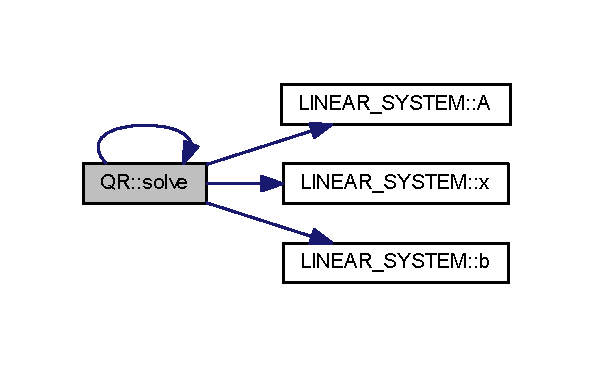
\includegraphics[width=285pt]{class_q_r_ab8f49cec36214bdcd9fca78e89c3737e_cgraph}
\end{center}
\end{figure}
Here is the caller graph for this function\+:\nopagebreak
\begin{figure}[H]
\begin{center}
\leavevmode
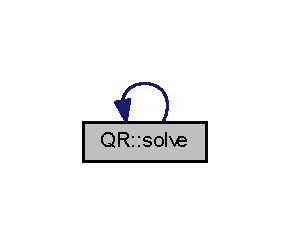
\includegraphics[width=139pt]{class_q_r_ab8f49cec36214bdcd9fca78e89c3737e_icgraph}
\end{center}
\end{figure}


The documentation for this class was generated from the following file\+:\begin{DoxyCompactItemize}
\item 
\mbox{\hyperlink{lin__sys_8h}{lin\+\_\+sys.\+h}}\end{DoxyCompactItemize}

\hypertarget{class_world_machine}{}\section{World\+Machine Class Reference}
\label{class_world_machine}\index{World\+Machine@{World\+Machine}}


C++ -\/ Q\+ML Schnittstelle Organisiert die Kaskade und das G\+UI.  




{\ttfamily \#include $<$World\+Machine.\+h$>$}



Inheritance diagram for World\+Machine\+:\nopagebreak
\begin{figure}[H]
\begin{center}
\leavevmode
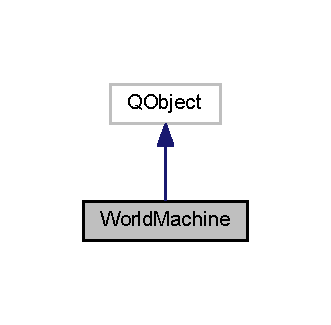
\includegraphics[width=159pt]{class_world_machine__inherit__graph}
\end{center}
\end{figure}


Collaboration diagram for World\+Machine\+:\nopagebreak
\begin{figure}[H]
\begin{center}
\leavevmode
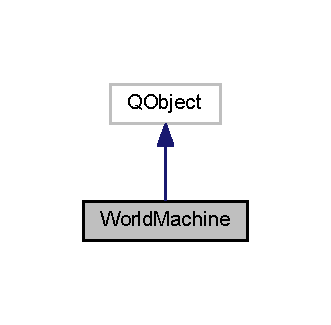
\includegraphics[width=159pt]{class_world_machine__coll__graph}
\end{center}
\end{figure}
\subsection*{Public Slots}
\begin{DoxyCompactItemize}
\item 
void \mbox{\hyperlink{class_world_machine_aa59dea1c70b3767e42a624daba7497b9}{start\+Cascade\+Slot}} ()
\item 
void \mbox{\hyperlink{class_world_machine_a0985510eda06d6ed11cab70c2cc234f1}{add\+Flash\+Slot}} (const int \&id)
\item 
void \mbox{\hyperlink{class_world_machine_abdd88afd0bef7ed98054e19cf59487c4}{delete\+Flash\+Slot}} (const int \&id)
\item 
void \mbox{\hyperlink{class_world_machine_adb2d5067594fa2f04f4c1035025ebe86}{connect\+Flashes\+Slot}} (const int \&id1, const int \&id2, const int \&phase)
\end{DoxyCompactItemize}
\subsection*{Public Member Functions}
\begin{DoxyCompactItemize}
\item 
\mbox{\hyperlink{class_world_machine_aafd4474fe539494cdb9a0e030a50d82c}{World\+Machine}} (Q\+Qml\+Application\+Engine $\ast$engine, Q\+Object $\ast$root)
\end{DoxyCompactItemize}


\subsection{Detailed Description}
C++ -\/ Q\+ML Schnittstelle Organisiert die Kaskade und das G\+UI. 

\subsection{Constructor \& Destructor Documentation}
\mbox{\Hypertarget{class_world_machine_aafd4474fe539494cdb9a0e030a50d82c}\label{class_world_machine_aafd4474fe539494cdb9a0e030a50d82c}} 
\index{World\+Machine@{World\+Machine}!World\+Machine@{World\+Machine}}
\index{World\+Machine@{World\+Machine}!World\+Machine@{World\+Machine}}
\subsubsection{\texorpdfstring{World\+Machine()}{WorldMachine()}}
{\footnotesize\ttfamily World\+Machine\+::\+World\+Machine (\begin{DoxyParamCaption}\item[{Q\+Qml\+Application\+Engine $\ast$}]{engine,  }\item[{Q\+Object $\ast$}]{root }\end{DoxyParamCaption})\hspace{0.3cm}{\ttfamily [inline]}}



\subsection{Member Function Documentation}
\mbox{\Hypertarget{class_world_machine_a0985510eda06d6ed11cab70c2cc234f1}\label{class_world_machine_a0985510eda06d6ed11cab70c2cc234f1}} 
\index{World\+Machine@{World\+Machine}!add\+Flash\+Slot@{add\+Flash\+Slot}}
\index{add\+Flash\+Slot@{add\+Flash\+Slot}!World\+Machine@{World\+Machine}}
\subsubsection{\texorpdfstring{add\+Flash\+Slot}{addFlashSlot}}
{\footnotesize\ttfamily void World\+Machine\+::add\+Flash\+Slot (\begin{DoxyParamCaption}\item[{const int \&}]{id }\end{DoxyParamCaption})\hspace{0.3cm}{\ttfamily [inline]}, {\ttfamily [slot]}}

Here is the call graph for this function\+:\nopagebreak
\begin{figure}[H]
\begin{center}
\leavevmode
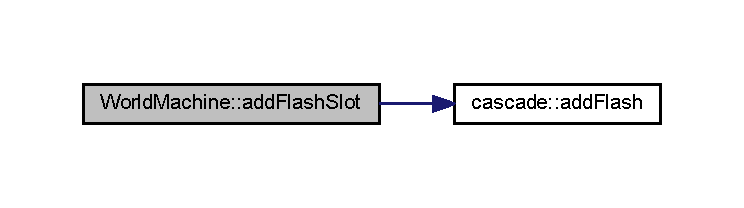
\includegraphics[width=350pt]{class_world_machine_a0985510eda06d6ed11cab70c2cc234f1_cgraph}
\end{center}
\end{figure}
\mbox{\Hypertarget{class_world_machine_adb2d5067594fa2f04f4c1035025ebe86}\label{class_world_machine_adb2d5067594fa2f04f4c1035025ebe86}} 
\index{World\+Machine@{World\+Machine}!connect\+Flashes\+Slot@{connect\+Flashes\+Slot}}
\index{connect\+Flashes\+Slot@{connect\+Flashes\+Slot}!World\+Machine@{World\+Machine}}
\subsubsection{\texorpdfstring{connect\+Flashes\+Slot}{connectFlashesSlot}}
{\footnotesize\ttfamily void World\+Machine\+::connect\+Flashes\+Slot (\begin{DoxyParamCaption}\item[{const int \&}]{id1,  }\item[{const int \&}]{id2,  }\item[{const int \&}]{phase }\end{DoxyParamCaption})\hspace{0.3cm}{\ttfamily [inline]}, {\ttfamily [slot]}}

Here is the call graph for this function\+:\nopagebreak
\begin{figure}[H]
\begin{center}
\leavevmode
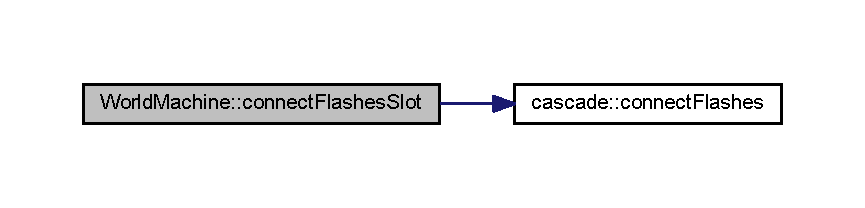
\includegraphics[width=350pt]{class_world_machine_adb2d5067594fa2f04f4c1035025ebe86_cgraph}
\end{center}
\end{figure}
\mbox{\Hypertarget{class_world_machine_abdd88afd0bef7ed98054e19cf59487c4}\label{class_world_machine_abdd88afd0bef7ed98054e19cf59487c4}} 
\index{World\+Machine@{World\+Machine}!delete\+Flash\+Slot@{delete\+Flash\+Slot}}
\index{delete\+Flash\+Slot@{delete\+Flash\+Slot}!World\+Machine@{World\+Machine}}
\subsubsection{\texorpdfstring{delete\+Flash\+Slot}{deleteFlashSlot}}
{\footnotesize\ttfamily void World\+Machine\+::delete\+Flash\+Slot (\begin{DoxyParamCaption}\item[{const int \&}]{id }\end{DoxyParamCaption})\hspace{0.3cm}{\ttfamily [inline]}, {\ttfamily [slot]}}

Here is the call graph for this function\+:\nopagebreak
\begin{figure}[H]
\begin{center}
\leavevmode
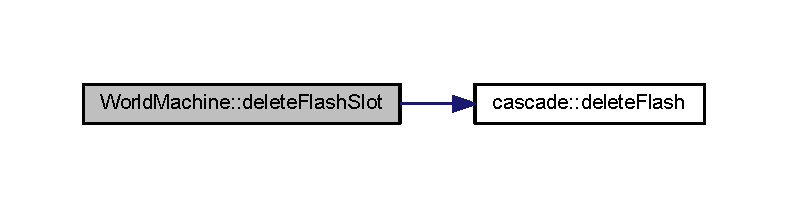
\includegraphics[width=350pt]{class_world_machine_abdd88afd0bef7ed98054e19cf59487c4_cgraph}
\end{center}
\end{figure}
\mbox{\Hypertarget{class_world_machine_aa59dea1c70b3767e42a624daba7497b9}\label{class_world_machine_aa59dea1c70b3767e42a624daba7497b9}} 
\index{World\+Machine@{World\+Machine}!start\+Cascade\+Slot@{start\+Cascade\+Slot}}
\index{start\+Cascade\+Slot@{start\+Cascade\+Slot}!World\+Machine@{World\+Machine}}
\subsubsection{\texorpdfstring{start\+Cascade\+Slot}{startCascadeSlot}}
{\footnotesize\ttfamily void World\+Machine\+::start\+Cascade\+Slot (\begin{DoxyParamCaption}{ }\end{DoxyParamCaption})\hspace{0.3cm}{\ttfamily [inline]}, {\ttfamily [slot]}}

Here is the call graph for this function\+:\nopagebreak
\begin{figure}[H]
\begin{center}
\leavevmode
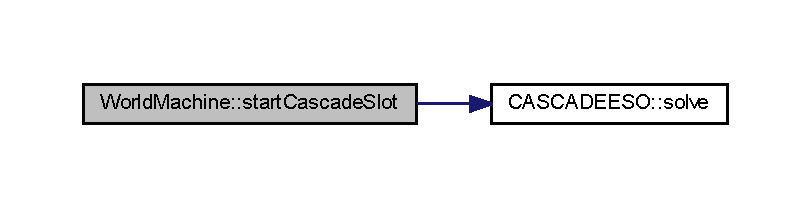
\includegraphics[width=350pt]{class_world_machine_aa59dea1c70b3767e42a624daba7497b9_cgraph}
\end{center}
\end{figure}


The documentation for this class was generated from the following file\+:\begin{DoxyCompactItemize}
\item 
\mbox{\hyperlink{_world_machine_8h}{World\+Machine.\+h}}\end{DoxyCompactItemize}

\chapter{File Documentation}
\hypertarget{cascade_8h}{}\section{cascade.\+h File Reference}
\label{cascade_8h}\index{cascade.\+h@{cascade.\+h}}


Enthält alle \mbox{\hyperlink{class_module}{Module}}.  


{\ttfamily \#include \char`\"{}flash.\+h\char`\"{}}\newline
{\ttfamily \#include $<$vector$>$}\newline
{\ttfamily \#include $<$Qt\+Core$>$}\newline
{\ttfamily \#include \char`\"{}dco/dco.\+hpp\char`\"{}}\newline
{\ttfamily \#include \char`\"{}Eso/\+Algebraic\+Eso\+View.\+hpp\char`\"{}}\newline
{\ttfamily \#include \char`\"{}Eso/\+Dco1\+Model.\+hpp\char`\"{}}\newline
{\ttfamily \#include \char`\"{}Eso/\+Eq\+Group.\+hpp\char`\"{}}\newline
{\ttfamily \#include \char`\"{}Eso/\+First\+Order\+Eso.\+hpp\char`\"{}}\newline
{\ttfamily \#include \char`\"{}Block\+Deco/\+Algebraic\+Eso\+Block\+Solver.\+hpp\char`\"{}}\newline
Include dependency graph for cascade.\+h\+:\nopagebreak
\begin{figure}[H]
\begin{center}
\leavevmode
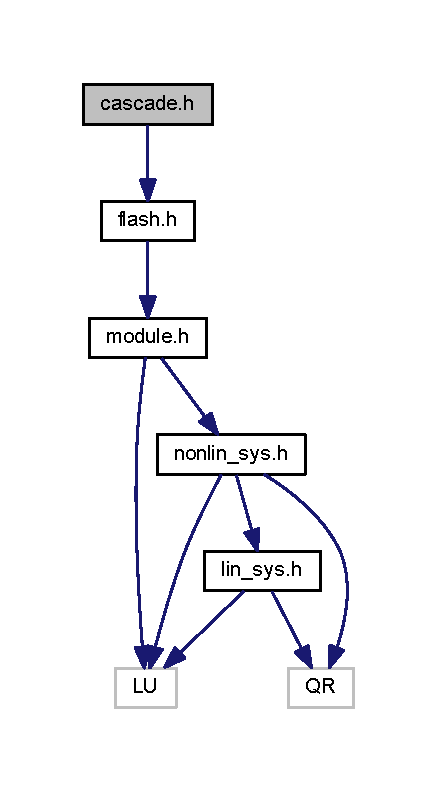
\includegraphics[width=350pt]{cascade_8h__incl}
\end{center}
\end{figure}
This graph shows which files directly or indirectly include this file\+:
\nopagebreak
\begin{figure}[H]
\begin{center}
\leavevmode
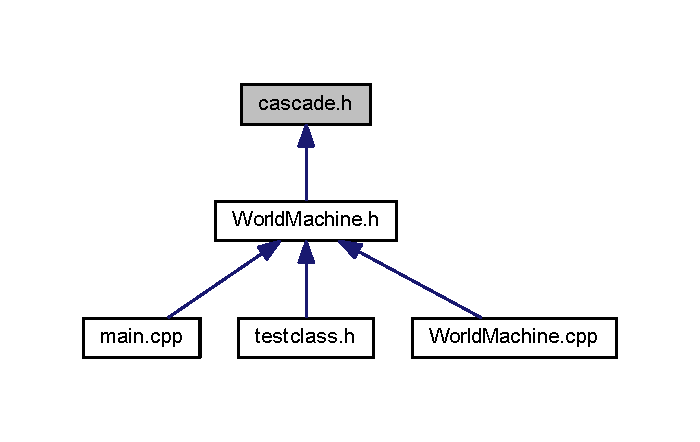
\includegraphics[width=167pt]{cascade_8h__dep__incl}
\end{center}
\end{figure}
\subsection*{Classes}
\begin{DoxyCompactItemize}
\item 
class \mbox{\hyperlink{classcascade}{cascade$<$ Real\+Type $>$}}
\begin{DoxyCompactList}\small\item\em Enthält alle Flashes. \end{DoxyCompactList}\item 
class \mbox{\hyperlink{class_c_a_s_c_a_d_e_e_s_o}{C\+A\+S\+C\+A\+D\+E\+E\+SO}}
\end{DoxyCompactItemize}
\subsection*{Typedefs}
\begin{DoxyCompactItemize}
\item 
{\footnotesize template$<$typename Real\+Type $>$ }\\using \mbox{\hyperlink{cascade_8h_a98b86f6842277476a0d5b3eaa896cec2}{Tangent\+Single\+Flash}} = Dco1\+Model$<$ \mbox{\hyperlink{classcascade}{cascade}}, Real\+Type $>$
\end{DoxyCompactItemize}


\subsection{Detailed Description}
Enthält alle \mbox{\hyperlink{class_module}{Module}}. 



\subsection{Typedef Documentation}
\mbox{\Hypertarget{cascade_8h_a98b86f6842277476a0d5b3eaa896cec2}\label{cascade_8h_a98b86f6842277476a0d5b3eaa896cec2}} 
\index{cascade.\+h@{cascade.\+h}!Tangent\+Single\+Flash@{Tangent\+Single\+Flash}}
\index{Tangent\+Single\+Flash@{Tangent\+Single\+Flash}!cascade.\+h@{cascade.\+h}}
\subsubsection{\texorpdfstring{Tangent\+Single\+Flash}{TangentSingleFlash}}
{\footnotesize\ttfamily template$<$typename Real\+Type $>$ \\
using \mbox{\hyperlink{cascade_8h_a98b86f6842277476a0d5b3eaa896cec2}{Tangent\+Single\+Flash}} =  Dco1\+Model$<$\mbox{\hyperlink{classcascade}{cascade}},Real\+Type$>$}


\hypertarget{flash_8h}{}\section{flash.\+h File Reference}
\label{flash_8h}\index{flash.\+h@{flash.\+h}}
{\ttfamily \#include \char`\"{}module.\+h\char`\"{}}\newline
Include dependency graph for flash.\+h\+:
\nopagebreak
\begin{figure}[H]
\begin{center}
\leavevmode
\includegraphics[width=136pt]{flash_8h__incl}
\end{center}
\end{figure}
This graph shows which files directly or indirectly include this file\+:
\nopagebreak
\begin{figure}[H]
\begin{center}
\leavevmode
\includegraphics[width=221pt]{flash_8h__dep__incl}
\end{center}
\end{figure}
\subsection*{Classes}
\begin{DoxyCompactItemize}
\item 
class \mbox{\hyperlink{class_flash}{Flash}}
\begin{DoxyCompactList}\small\item\em Flashmodul. \end{DoxyCompactList}\end{DoxyCompactItemize}

\hypertarget{lin__sys_8h}{}\section{lin\+\_\+sys.\+h File Reference}
\label{lin__sys_8h}\index{lin\+\_\+sys.\+h@{lin\+\_\+sys.\+h}}


Lineare Systeme.  


{\ttfamily \#include \char`\"{}LU\char`\"{}}\newline
{\ttfamily \#include \char`\"{}QR\char`\"{}}\newline
Include dependency graph for lin\+\_\+sys.\+h\+:\nopagebreak
\begin{figure}[H]
\begin{center}
\leavevmode
\includegraphics[width=158pt]{lin__sys_8h__incl}
\end{center}
\end{figure}
This graph shows which files directly or indirectly include this file\+:
\nopagebreak
\begin{figure}[H]
\begin{center}
\leavevmode
\includegraphics[width=336pt]{lin__sys_8h__dep__incl}
\end{center}
\end{figure}
\subsection*{Classes}
\begin{DoxyCompactItemize}
\item 
class \mbox{\hyperlink{class_l_i_n_e_a_r___s_y_s_t_e_m}{L\+I\+N\+E\+A\+R\+\_\+\+S\+Y\+S\+T\+E\+M$<$ T\+A, N, Tb, Tx $>$}}
\begin{DoxyCompactList}\small\item\em Lineare Systeme Basierend auf \mbox{\hyperlink{lin__sys_8h}{lin\+\_\+sys.\+h}} von Uwe Naumann. \end{DoxyCompactList}\item 
class \mbox{\hyperlink{class_l_i_n_e_a_r___s_o_l_v_e_r}{L\+I\+N\+E\+A\+R\+\_\+\+S\+O\+L\+V\+E\+R$<$ T\+A, N, Tb, Tx $>$}}
\item 
class \mbox{\hyperlink{class_l_u}{L\+U$<$ T\+A, N, Tb, Tx $>$}}
\item 
class \mbox{\hyperlink{class_q_r}{Q\+R$<$ T\+A, N, Tb, Tx $>$}}
\end{DoxyCompactItemize}


\subsection{Detailed Description}
Lineare Systeme. 


\hypertarget{main_8cpp}{}\section{main.\+cpp File Reference}
\label{main_8cpp}\index{main.\+cpp@{main.\+cpp}}


Programminitiation.  


{\ttfamily \#include \char`\"{}World\+Machine.\+h\char`\"{}}\newline
{\ttfamily \#include $<$Q\+Gui\+Application$>$}\newline
{\ttfamily \#include $<$Qt\+Qml/\+Q\+Qml\+Application\+Engine$>$}\newline
{\ttfamily \#include $<$Qt\+Qml/\+Q\+Qml\+Engine$>$}\newline
Include dependency graph for main.\+cpp\+:\nopagebreak
\begin{figure}[H]
\begin{center}
\leavevmode
\includegraphics[width=350pt]{main_8cpp__incl}
\end{center}
\end{figure}
\subsection*{Functions}
\begin{DoxyCompactItemize}
\item 
int \mbox{\hyperlink{main_8cpp_a0ddf1224851353fc92bfbff6f499fa97}{main}} (int argc, char $\ast$argv\mbox{[}$\,$\mbox{]})
\end{DoxyCompactItemize}


\subsection{Detailed Description}
Programminitiation. 


\begin{DoxyParams}{Parameters}
{\em argc} & dummy \\
\hline
{\em argv} & dummy \\
\hline
\end{DoxyParams}


\subsection{Function Documentation}
\mbox{\Hypertarget{main_8cpp_a0ddf1224851353fc92bfbff6f499fa97}\label{main_8cpp_a0ddf1224851353fc92bfbff6f499fa97}} 
\index{main.\+cpp@{main.\+cpp}!main@{main}}
\index{main@{main}!main.\+cpp@{main.\+cpp}}
\subsubsection{\texorpdfstring{main()}{main()}}
{\footnotesize\ttfamily int main (\begin{DoxyParamCaption}\item[{int}]{argc,  }\item[{char $\ast$}]{argv\mbox{[}$\,$\mbox{]} }\end{DoxyParamCaption})}


\hypertarget{module_8h}{}\section{module.\+h File Reference}
\label{module_8h}\index{module.\+h@{module.\+h}}


Basismodul.  


{\ttfamily \#include \char`\"{}LU\char`\"{}}\newline
{\ttfamily \#include \char`\"{}QR\char`\"{}}\newline
{\ttfamily \#include \char`\"{}lin\+\_\+sys.\+h\char`\"{}}\newline
{\ttfamily \#include $<$iostream$>$}\newline
Include dependency graph for module.\+h\+:\nopagebreak
\begin{figure}[H]
\begin{center}
\leavevmode
\includegraphics[width=285pt]{module_8h__incl}
\end{center}
\end{figure}
This graph shows which files directly or indirectly include this file\+:
\nopagebreak
\begin{figure}[H]
\begin{center}
\leavevmode
\includegraphics[width=336pt]{module_8h__dep__incl}
\end{center}
\end{figure}
\subsection*{Classes}
\begin{DoxyCompactItemize}
\item 
class \mbox{\hyperlink{class_module}{Module$<$ T\+S, N\+P, N\+S, T\+P $>$}}
\begin{DoxyCompactList}\small\item\em Akstrakte Klasse für allgemeine Bauteile. \end{DoxyCompactList}\item 
class \mbox{\hyperlink{class_m_o_d_u_l_e_n_e_w_t_o_n}{M\+O\+D\+U\+L\+E\+N\+E\+W\+T\+O\+N$<$ T\+S, N\+P, N\+S, T\+P $>$}}
\begin{DoxyCompactList}\small\item\em Newton Löser für Abgeleitete Klassen von Modul. \end{DoxyCompactList}\end{DoxyCompactItemize}


\subsection{Detailed Description}
Basismodul. 


\hypertarget{nonlin__sys_8h}{}\section{nonlin\+\_\+sys.\+h File Reference}
\label{nonlin__sys_8h}\index{nonlin\+\_\+sys.\+h@{nonlin\+\_\+sys.\+h}}


Nichtlineare Systeme.  


{\ttfamily \#include \char`\"{}LU\char`\"{}}\newline
{\ttfamily \#include \char`\"{}QR\char`\"{}}\newline
{\ttfamily \#include \char`\"{}lin\+\_\+sys.\+h\char`\"{}}\newline
{\ttfamily \#include $<$iostream$>$}\newline
Include dependency graph for nonlin\+\_\+sys.\+h\+:\nopagebreak
\begin{figure}[H]
\begin{center}
\leavevmode
\includegraphics[width=305pt]{nonlin__sys_8h__incl}
\end{center}
\end{figure}
\subsection*{Classes}
\begin{DoxyCompactItemize}
\item 
class \mbox{\hyperlink{class_n_o_n_l_i_n_e_a_r___s_y_s_t_e_m}{N\+O\+N\+L\+I\+N\+E\+A\+R\+\_\+\+S\+Y\+S\+T\+E\+M$<$ T\+S, N\+P, N\+S, T\+P $>$}}
\begin{DoxyCompactList}\small\item\em Nichtlineare Systeme Basierend auf \mbox{\hyperlink{nonlin__sys_8h}{nonlin\+\_\+sys.\+h}} von Uwe Naumann. \end{DoxyCompactList}\item 
class \mbox{\hyperlink{class_n_o_n_l_i_n_e_a_r___s_o_l_v_e_r}{N\+O\+N\+L\+I\+N\+E\+A\+R\+\_\+\+S\+O\+L\+V\+E\+R$<$ T\+S, N\+P, N\+S, T\+P $>$}}
\item 
class \mbox{\hyperlink{class_n_e_w_t_o_n}{N\+E\+W\+T\+O\+N$<$ T\+S, N\+P, N\+S, T\+P $>$}}
\end{DoxyCompactItemize}


\subsection{Detailed Description}
Nichtlineare Systeme. 


\hypertarget{_world_machine_8h}{}\section{World\+Machine.\+h File Reference}
\label{_world_machine_8h}\index{World\+Machine.\+h@{World\+Machine.\+h}}


C++ -\/ Q\+ML Schnittstelle.  


{\ttfamily \#include $<$Qt\+Core$>$}\newline
{\ttfamily \#include \char`\"{}cascade.\+h\char`\"{}}\newline
Include dependency graph for World\+Machine.\+h\+:\nopagebreak
\begin{figure}[H]
\begin{center}
\leavevmode
\includegraphics[width=316pt]{_world_machine_8h__incl}
\end{center}
\end{figure}
This graph shows which files directly or indirectly include this file\+:
\nopagebreak
\begin{figure}[H]
\begin{center}
\leavevmode
\includegraphics[width=336pt]{_world_machine_8h__dep__incl}
\end{center}
\end{figure}
\subsection*{Classes}
\begin{DoxyCompactItemize}
\item 
class \mbox{\hyperlink{class_world_machine}{World\+Machine}}
\begin{DoxyCompactList}\small\item\em C++ -\/ Q\+ML Schnittstelle Organisiert die Kaskade und das G\+UI. \end{DoxyCompactList}\end{DoxyCompactItemize}


\subsection{Detailed Description}
C++ -\/ Q\+ML Schnittstelle. 


%--- End generated contents ---

% Index
\backmatter
\newpage
\phantomsection
\clearemptydoublepage
\addcontentsline{toc}{chapter}{Index}
\printindex

\end{document}
